\documentclass[]{book}
\usepackage{lmodern}
\usepackage{amssymb,amsmath}
\usepackage{ifxetex,ifluatex}
\usepackage{fixltx2e} % provides \textsubscript
\ifnum 0\ifxetex 1\fi\ifluatex 1\fi=0 % if pdftex
  \usepackage[T1]{fontenc}
  \usepackage[utf8]{inputenc}
\else % if luatex or xelatex
  \ifxetex
    \usepackage{mathspec}
  \else
    \usepackage{fontspec}
  \fi
  \defaultfontfeatures{Ligatures=TeX,Scale=MatchLowercase}
\fi
% use upquote if available, for straight quotes in verbatim environments
\IfFileExists{upquote.sty}{\usepackage{upquote}}{}
% use microtype if available
\IfFileExists{microtype.sty}{%
\usepackage{microtype}
\UseMicrotypeSet[protrusion]{basicmath} % disable protrusion for tt fonts
}{}
\usepackage{hyperref}
\hypersetup{unicode=true,
            pdftitle={Software R para avaliação de dados experimentais},
            pdfauthor={Tiago Olivoto},
            pdfborder={0 0 0},
            breaklinks=true}
\urlstyle{same}  % don't use monospace font for urls
\usepackage{natbib}
\bibliographystyle{apalike}
\usepackage{color}
\usepackage{fancyvrb}
\newcommand{\VerbBar}{|}
\newcommand{\VERB}{\Verb[commandchars=\\\{\}]}
\DefineVerbatimEnvironment{Highlighting}{Verbatim}{commandchars=\\\{\}}
% Add ',fontsize=\small' for more characters per line
\usepackage{framed}
\definecolor{shadecolor}{RGB}{248,248,248}
\newenvironment{Shaded}{\begin{snugshade}}{\end{snugshade}}
\newcommand{\AlertTok}[1]{\textcolor[rgb]{0.94,0.16,0.16}{#1}}
\newcommand{\AnnotationTok}[1]{\textcolor[rgb]{0.56,0.35,0.01}{\textbf{\textit{#1}}}}
\newcommand{\AttributeTok}[1]{\textcolor[rgb]{0.77,0.63,0.00}{#1}}
\newcommand{\BaseNTok}[1]{\textcolor[rgb]{0.00,0.00,0.81}{#1}}
\newcommand{\BuiltInTok}[1]{#1}
\newcommand{\CharTok}[1]{\textcolor[rgb]{0.31,0.60,0.02}{#1}}
\newcommand{\CommentTok}[1]{\textcolor[rgb]{0.56,0.35,0.01}{\textit{#1}}}
\newcommand{\CommentVarTok}[1]{\textcolor[rgb]{0.56,0.35,0.01}{\textbf{\textit{#1}}}}
\newcommand{\ConstantTok}[1]{\textcolor[rgb]{0.00,0.00,0.00}{#1}}
\newcommand{\ControlFlowTok}[1]{\textcolor[rgb]{0.13,0.29,0.53}{\textbf{#1}}}
\newcommand{\DataTypeTok}[1]{\textcolor[rgb]{0.13,0.29,0.53}{#1}}
\newcommand{\DecValTok}[1]{\textcolor[rgb]{0.00,0.00,0.81}{#1}}
\newcommand{\DocumentationTok}[1]{\textcolor[rgb]{0.56,0.35,0.01}{\textbf{\textit{#1}}}}
\newcommand{\ErrorTok}[1]{\textcolor[rgb]{0.64,0.00,0.00}{\textbf{#1}}}
\newcommand{\ExtensionTok}[1]{#1}
\newcommand{\FloatTok}[1]{\textcolor[rgb]{0.00,0.00,0.81}{#1}}
\newcommand{\FunctionTok}[1]{\textcolor[rgb]{0.00,0.00,0.00}{#1}}
\newcommand{\ImportTok}[1]{#1}
\newcommand{\InformationTok}[1]{\textcolor[rgb]{0.56,0.35,0.01}{\textbf{\textit{#1}}}}
\newcommand{\KeywordTok}[1]{\textcolor[rgb]{0.13,0.29,0.53}{\textbf{#1}}}
\newcommand{\NormalTok}[1]{#1}
\newcommand{\OperatorTok}[1]{\textcolor[rgb]{0.81,0.36,0.00}{\textbf{#1}}}
\newcommand{\OtherTok}[1]{\textcolor[rgb]{0.56,0.35,0.01}{#1}}
\newcommand{\PreprocessorTok}[1]{\textcolor[rgb]{0.56,0.35,0.01}{\textit{#1}}}
\newcommand{\RegionMarkerTok}[1]{#1}
\newcommand{\SpecialCharTok}[1]{\textcolor[rgb]{0.00,0.00,0.00}{#1}}
\newcommand{\SpecialStringTok}[1]{\textcolor[rgb]{0.31,0.60,0.02}{#1}}
\newcommand{\StringTok}[1]{\textcolor[rgb]{0.31,0.60,0.02}{#1}}
\newcommand{\VariableTok}[1]{\textcolor[rgb]{0.00,0.00,0.00}{#1}}
\newcommand{\VerbatimStringTok}[1]{\textcolor[rgb]{0.31,0.60,0.02}{#1}}
\newcommand{\WarningTok}[1]{\textcolor[rgb]{0.56,0.35,0.01}{\textbf{\textit{#1}}}}
\usepackage{longtable,booktabs}
\usepackage{graphicx,grffile}
\makeatletter
\def\maxwidth{\ifdim\Gin@nat@width>\linewidth\linewidth\else\Gin@nat@width\fi}
\def\maxheight{\ifdim\Gin@nat@height>\textheight\textheight\else\Gin@nat@height\fi}
\makeatother
% Scale images if necessary, so that they will not overflow the page
% margins by default, and it is still possible to overwrite the defaults
% using explicit options in \includegraphics[width, height, ...]{}
\setkeys{Gin}{width=\maxwidth,height=\maxheight,keepaspectratio}
\IfFileExists{parskip.sty}{%
\usepackage{parskip}
}{% else
\setlength{\parindent}{0pt}
\setlength{\parskip}{6pt plus 2pt minus 1pt}
}
\setlength{\emergencystretch}{3em}  % prevent overfull lines
\providecommand{\tightlist}{%
  \setlength{\itemsep}{0pt}\setlength{\parskip}{0pt}}
\setcounter{secnumdepth}{5}
% Redefines (sub)paragraphs to behave more like sections
\ifx\paragraph\undefined\else
\let\oldparagraph\paragraph
\renewcommand{\paragraph}[1]{\oldparagraph{#1}\mbox{}}
\fi
\ifx\subparagraph\undefined\else
\let\oldsubparagraph\subparagraph
\renewcommand{\subparagraph}[1]{\oldsubparagraph{#1}\mbox{}}
\fi

%%% Use protect on footnotes to avoid problems with footnotes in titles
\let\rmarkdownfootnote\footnote%
\def\footnote{\protect\rmarkdownfootnote}

%%% Change title format to be more compact
\usepackage{titling}

% Create subtitle command for use in maketitle
\providecommand{\subtitle}[1]{
  \posttitle{
    \begin{center}\large#1\end{center}
    }
}

\setlength{\droptitle}{-2em}

  \title{Software R para avaliação de dados experimentais}
    \pretitle{\vspace{\droptitle}\centering\huge}
  \posttitle{\par}
  \subtitle{Um foco em experimentos agronômicos}
  \author{Tiago Olivoto}
    \preauthor{\centering\large\emph}
  \postauthor{\par}
      \predate{\centering\large\emph}
  \postdate{\par}
    \date{2019-08-14}

\usepackage{booktabs}
\usepackage{amsthm}
\usepackage{bm}
\makeatletter
\def\thm@space@setup{%
  \thm@preskip=8pt plus 2pt minus 4pt
  \thm@postskip=\thm@preskip
}
\makeatother
\usepackage{imakeidx}
\makeindex[program=makeindex, name=function, title=Índice de códigos R, options=-s pyro,columns=3,intoc=true]
\makeindex[program=makeindex, title=Índice de texto, options=-s pyro,columns=3,intoc=true]
\newcommand{\ST}[1]{\textbf{\hyperpage{#1}}\normalsize}
\newcommand{\indf}[1]{\index[function]{#1@\texttt{#1()}|ST}}
\newcommand{\indt}[1]{\index{#1|ST}}

\newenvironment{tarefa}
  {\begin{customBlockImage}[colframe=customOrange, title=Tarefa de casa]{images/head}}
  {\end{customBlockImage}}

\begin{document}
\maketitle

{
\setcounter{tocdepth}{1}
\tableofcontents
}
\hypertarget{prefacio}{%
\chapter*{Préfácio}\label{prefacio}}
\addcontentsline{toc}{chapter}{Préfácio}

Atualmente na área das Ciências Agrárias identificam-se o uso de diversos sofware para a análise estatística de dados originados em coletas de experimentos. Esta miscelânea de sofware pode confundir o pesquisador no momento de escolher qual é o software que será adotado para suas análises estatísticas, já que existem aqueles que devem ser adquiridas licenças para uso e nem todos disponibilizam opções de todos os métodos de análise estatística de dados.

Dentre esses, o R (R Development Core Team, 2008) destaca-se por ser uma
linguagem de programação de código aberto (open source) basicamente destinado para computação estatística e gráficos. Com a proposta de organização de um curso e capacitação de acadêmicos e professores envolvidos em Pós-Graduação na Área de Ciências Agrárias, os Drs. Bruno Giacomini Sari e Tiago Olivoto propuseram-se a elaborar um documento onde oferecem uma excelente apresentação e introdução ao ambiente R, bem como diversas aplicações de abordagens estatísticas em experimentos agrícolas.

Assim este documento é uma resenha da introdução ao uso do R, bem como de modelos de análise e interpretação de experimentos agrícolas. Apresentam-se variações nos tipos de tratamentos (qualitativos e quantitativos), variações nos desdobramentos das interações e variações nas formas da casualização de experimentos bifatoriais. Seu intuito não é ensinar estatística. A expectativa é de que este documento seja útil para aqueles pesquisadores que desejam utilizar este ambiente de programação para a realização de suas análises estatísticas e que sirva de consulta para o planejamento de experimentos com diferentes casualizações dos tratamentos.

Parabenizamos os autores pela iniciativa e qualidade do material oferecido.

Alessandro Dal'Col Lúcio
Professor Titular, Setor de Experimentação Vegetal
Departamento de Fitotecnia
Centro de Ciências Rurais
Universidade Federal de Santa Maria

\hypertarget{por-que-deveria-ler-esta-apostila}{%
\chapter*{Por que deveria ler esta apostila}\label{por-que-deveria-ler-esta-apostila}}
\addcontentsline{toc}{chapter}{Por que deveria ler esta apostila}

Com uma disponibilidade cada vez maior de bons softwares estatísticos, a escolha por um único programa se torna uma tarefa difícil, até mesmo para alguém com vasta experiência na área de análise de dados de experimentos agronômicos. O ambiente de programação R é, também, um poderoso software estatístico. Assim, inúmeras são as fontes com informações relacionadas a análise de dados, criação de gráficos, etc.

A grande maioria dos blogs\footnote{\url{http://www.sthda.com/english/wiki/easy-r-programming-basics}} \footnote{\url{http://www.sthda.com/english/wiki/data-visualization}} \footnote{\url{http://www.sthda.com/english/wiki/r-basic-statistics}} \footnote{\url{https://ggplot2.tidyverse.org/}} \footnote{\url{https://stats.stackexchange.com/}} \footnote{\url{https://www.r-graph-gallery.com/}} \footnote{\url{https://www.r-graph-gallery.com/}} \footnote{\url{https://www.r-bloggers.com}} relacionados ao software R estão na língua Inglesa e mesmo que nos tempos atuais esta não seja uma questão limitante, materiais de qualidade em língua Portuguesa são muito bem-vindos. Por exemplo, a \href{http://r-br.2285057.n4.nabble.com/}{R-br} \footnote{\url{http://r-br.2285057.n4.nabble.com/}} é a lista Brasileira oficial de discussão do programa R e tem o propósito de permitir a troca de informações entre os usuários de R (em português) e contém inúmeras dicas/discussões sobre as mais diversas áreas de estudo.

Esta apostila, voltada para a análise de dados de experimentos agronômicos, apresenta a teoria e a aplicação no software R dos procedimentos mais utilizados na análise de experimentos agronômicos. Assim, ela pode servir de referência para aqueles que querem realizar suas análises no R, principalmente para os que ainda possuem pouca ou nenhuma experiência com este ambiente de programação.

Os leitores podem interagir com os exemplos deste material ao lê-lo? Isto será difícil se o material for impresso em papel, mas é perfeitamente possível em sua versão digital utilizando \texttt{Ctrl+C} e \texttt{Ctrl+V}. Por exemplo, é possível copiar uma programação, colar em seu ambiente de trabalho e saber imediatamente o que acontece se certos parâmetros de um modelo/análise forem alterados.

\hypertarget{estrutura-da-apostila}{%
\chapter*{Estrutura da apostila}\label{estrutura-da-apostila}}
\addcontentsline{toc}{chapter}{Estrutura da apostila}

Esta apostila contém 14 capítulos divididos em 3 grandes partes. Na parte I (Capítulos 1 a 5 ) o ambiente R é apresentado. O \protect\hyperlink{intro}{Capítulo 1}, apresenta uma breve introdução sobre os softwares R e RStudio, mostrando como instalar e carregar os pacotes necessários, além de mostrar ao leitor como criar seu primeiro script. O \protect\hyperlink{objects}{Capítulo 2} apresenta os tipos de objetos. No \protect\hyperlink{math}{Capítulo 3}, as principais operações matemáticas são mostradas. No \protect\hyperlink{loops}{Capítulo 4} é mostrado como \emph{loops} podem ser úteis para repetir um determinado código diversas vezes. No \protect\hyperlink{dataframe}{Capítulo 5} é mostrado os dados podem ser armazenados em objetos com diferentes classes.

A parte II (Capítulos 6 a 9) é voltada para a organização, manipulação e apresentação gráfica de dados. No \protect\hyperlink{entrada}{Capítulo 6} é mostrado diversos formatos de dados podem ser carregados no ambiente R. O \protect\hyperlink{manipula}{Capítulo 7} trata da manimulação dos dados, tais como adição, seleção, resumo e combinação de variáveis. O \protect\hyperlink{graph}{Capítulo 8} trata da apresentação dos dados utilizando diversos tipos de gráficos, tais como barra, histogramas e gráficos de dispersão. O \protect\hyperlink{exporta}{Capítulo 9} é voltado para a exportação dos dados, tanto numérico quanto gráficos.

A parte III (Capítulos 10 a 14) é voltada para a análise dos dados. O \protect\hyperlink{analdata}{Capítulo 10} trata da análise de dados experimentais, incluindo a estatística básica, análise de experimentos uni- e bi-fatoriais considerando os principais delineamentos, transformações de dados, análise de covariância bem como uma breve abordagem ao uso de modelos lineares generalizados. O \protect\hyperlink{reg}{Capítulo 11} é voltado exclusivamente para análise de regressão linear e não linear. O \protect\hyperlink{relations}{Capítulo 12} trata da associação entre variáveis tais como correlação linear, correlação parcial e análise de trilha. No \protect\hyperlink{multivariate}{Capítulo 13} a análise multivariada de dados é apresentada. Por fim --mas não menos importante-- no \protect\hyperlink{interaction}{Capítulo 14} são apresentados diversos modelos para análise de ensaios multi-ambientes, com ênfase na aplicação dos métodos AMMI\footnote{Additive Main Effect and Multiplicative Interaction}, BLUP\footnote{Best Linear Unbiased Prediction} e GGE\footnote{Genotype plus Genotype-vs-Environment Interaction}.

\hypertarget{intro}{%
\chapter{\texorpdfstring{Introdução ao ambiente \emph{R}}{Introdução ao ambiente R}}\label{intro}}

\hypertarget{o-software-r}{%
\section{O software R}\label{o-software-r}}

O artigo \href{https://www.jstor.org/stable/1390807?seq=1\#page_scan_tab_contents}{R: A Language for Data Analysis and Graphics}\footnote{\url{https://www.jstor.org/stable/1390807?seq=1\#page_scan_tab_contents}} marca o início de uma nova era no processamento e análise de dados: o desenvolvimento do software R. O R é uma linguagem e ambiente estatístico que traz muitas vantagens para o usuário, embora elas não sejam tão obvias inicialmente: (i) o R é um Software Livre (livre no sentido de liberdade) distribuído sob a \href{https://www.gnu.org/licenses/quick-guide-gplv3.html}{Licença Pública Geral}\footnote{\url{https://www.gnu.org/licenses/quick-guide-gplv3.html}}, podendo ser livremente copiado, distribuído, e instalado em diversos computadores livremente. Isso contrasta com softwares comerciais, que têm licenças altamente restritivas, que não permitem que cópias sejam distribuídas ou instaladas em mais de um computador sem a devida licença (que obviamente é paga!); (ii) a grande maioria dos Softwares livres são grátis, e o R não é uma exceção; (iii) os códigos-fontes R estão disponíveis para os usuários, e atualmente são gerenciados por um grupo chamado \href{https://www.r-project.org/}{R Development Core Team}\footnote{\url{https://www.r-project.org/}}. A vantagem de ter o código aberto é que falhas podem ser detectadas e rapidamente corrigidas. Este sistema de revisão depende da participação dos usuários. Em contraste, em muitos pacotes comerciais, as falhas não são corrigidas até o lançamento da próxima versão, o que pode levar vários anos; (iv) o R fornece um interface de entrada por linha de comando (ELC).

No \indt{software} R, todos os comandos são digitados e o mouse é pouco usado. Pode parecer antigo, pouco amigável ou até pobre em recursos visuais, mas isso faz com que nos deparemos com o melhor recurso do R: a sua flexibilidade. Para usuários familiarizados, a linguagem do R se torna clara e simples. Com poucos comandos, funções poderosas podem ser criadas e o usuário é sempre consciente do que foi pedido através da ELC (Meus dados, minhas análises!). Isso contrasta com pacotes que possuem uma interface amigável (Windows-based), mas escondem a dinâmica dos cálculos e, potencialmente, os seus erros. Finalmente, o R fornece uma ampla variedade de procedimentos estatísticos básicos ou que exigem grande esforço computacional (modelagem linear e não linear, testes estatísticos clássicos, análise de séries temporais, classificação, agrupamento, etc.) e recursos gráficos elegantes. Um dos pontos fortes de R é a facilidade com que gráficos de qualidade podem ser produzidos, incluindo símbolos matemáticos e fórmulas, quando necessário. O software R está disponível em uma ampla variedade de plataformas UNIX e sistemas similares (incluindo FreeBSD e Linux), Windows e MacOS.

\hypertarget{o-software-rstudio}{%
\section{O software RStudio}\label{o-software-rstudio}}

Quem ja é usuário de softwares por linhas de comando, como o SAS, provavelmente não notou nenhuma grande diferença até aqui. Toda análise se resume à seguinte sequência \emph{dados \textgreater{} códigos \textgreater{} saída}. A experiência do usuário com o R, no entanto, pode ser mais atrativa utilizando o \href{https://www.rstudio.com/}{RStudio}\footnote{\url{https://www.rstudio.com/}}. O Rstudio é um produto de código aberto disponível publicamente em 28/02/2011 que está disponível gratuitamente. Ele é um ambiente de desenvolvimento integrado para R que inclui (i) janelas de edição de texto a partir das quais o código pode ser enviado para o console e/ou salvo no sistema operacional, (ii) listas de objetos em sua área de trabalho, (iii) histórico infinito dos comandos facilmente pesquisável com capacidade de inserir, a partir do histórico, um comando no console novamente; (iv); interface com o sistema operacional para acesso a arquivos; (v) janela de ajuda com botões de voltar e avançar; (vi) download de pacotes. Apesar de todas estas capacidades, o RStudio é muito fácil de utilizar.

Nesta seção serão abordados alguns aspectos básicos para que o usuário do R possa desenvolver as suas análises. Será dado enfoque para áreas básicas da interface, cujo conhecimento é necessário para que um usuário inicante possa realizar sua primeira análisee. A figura abaixo mostra as principais janelas do \textbf{Rstudio}, incluindo o \emph{script}, o \emph{console}, a \emph{``área de trabalho''} e o \emph{output} para gráficos.

\begin{figure}
\centering
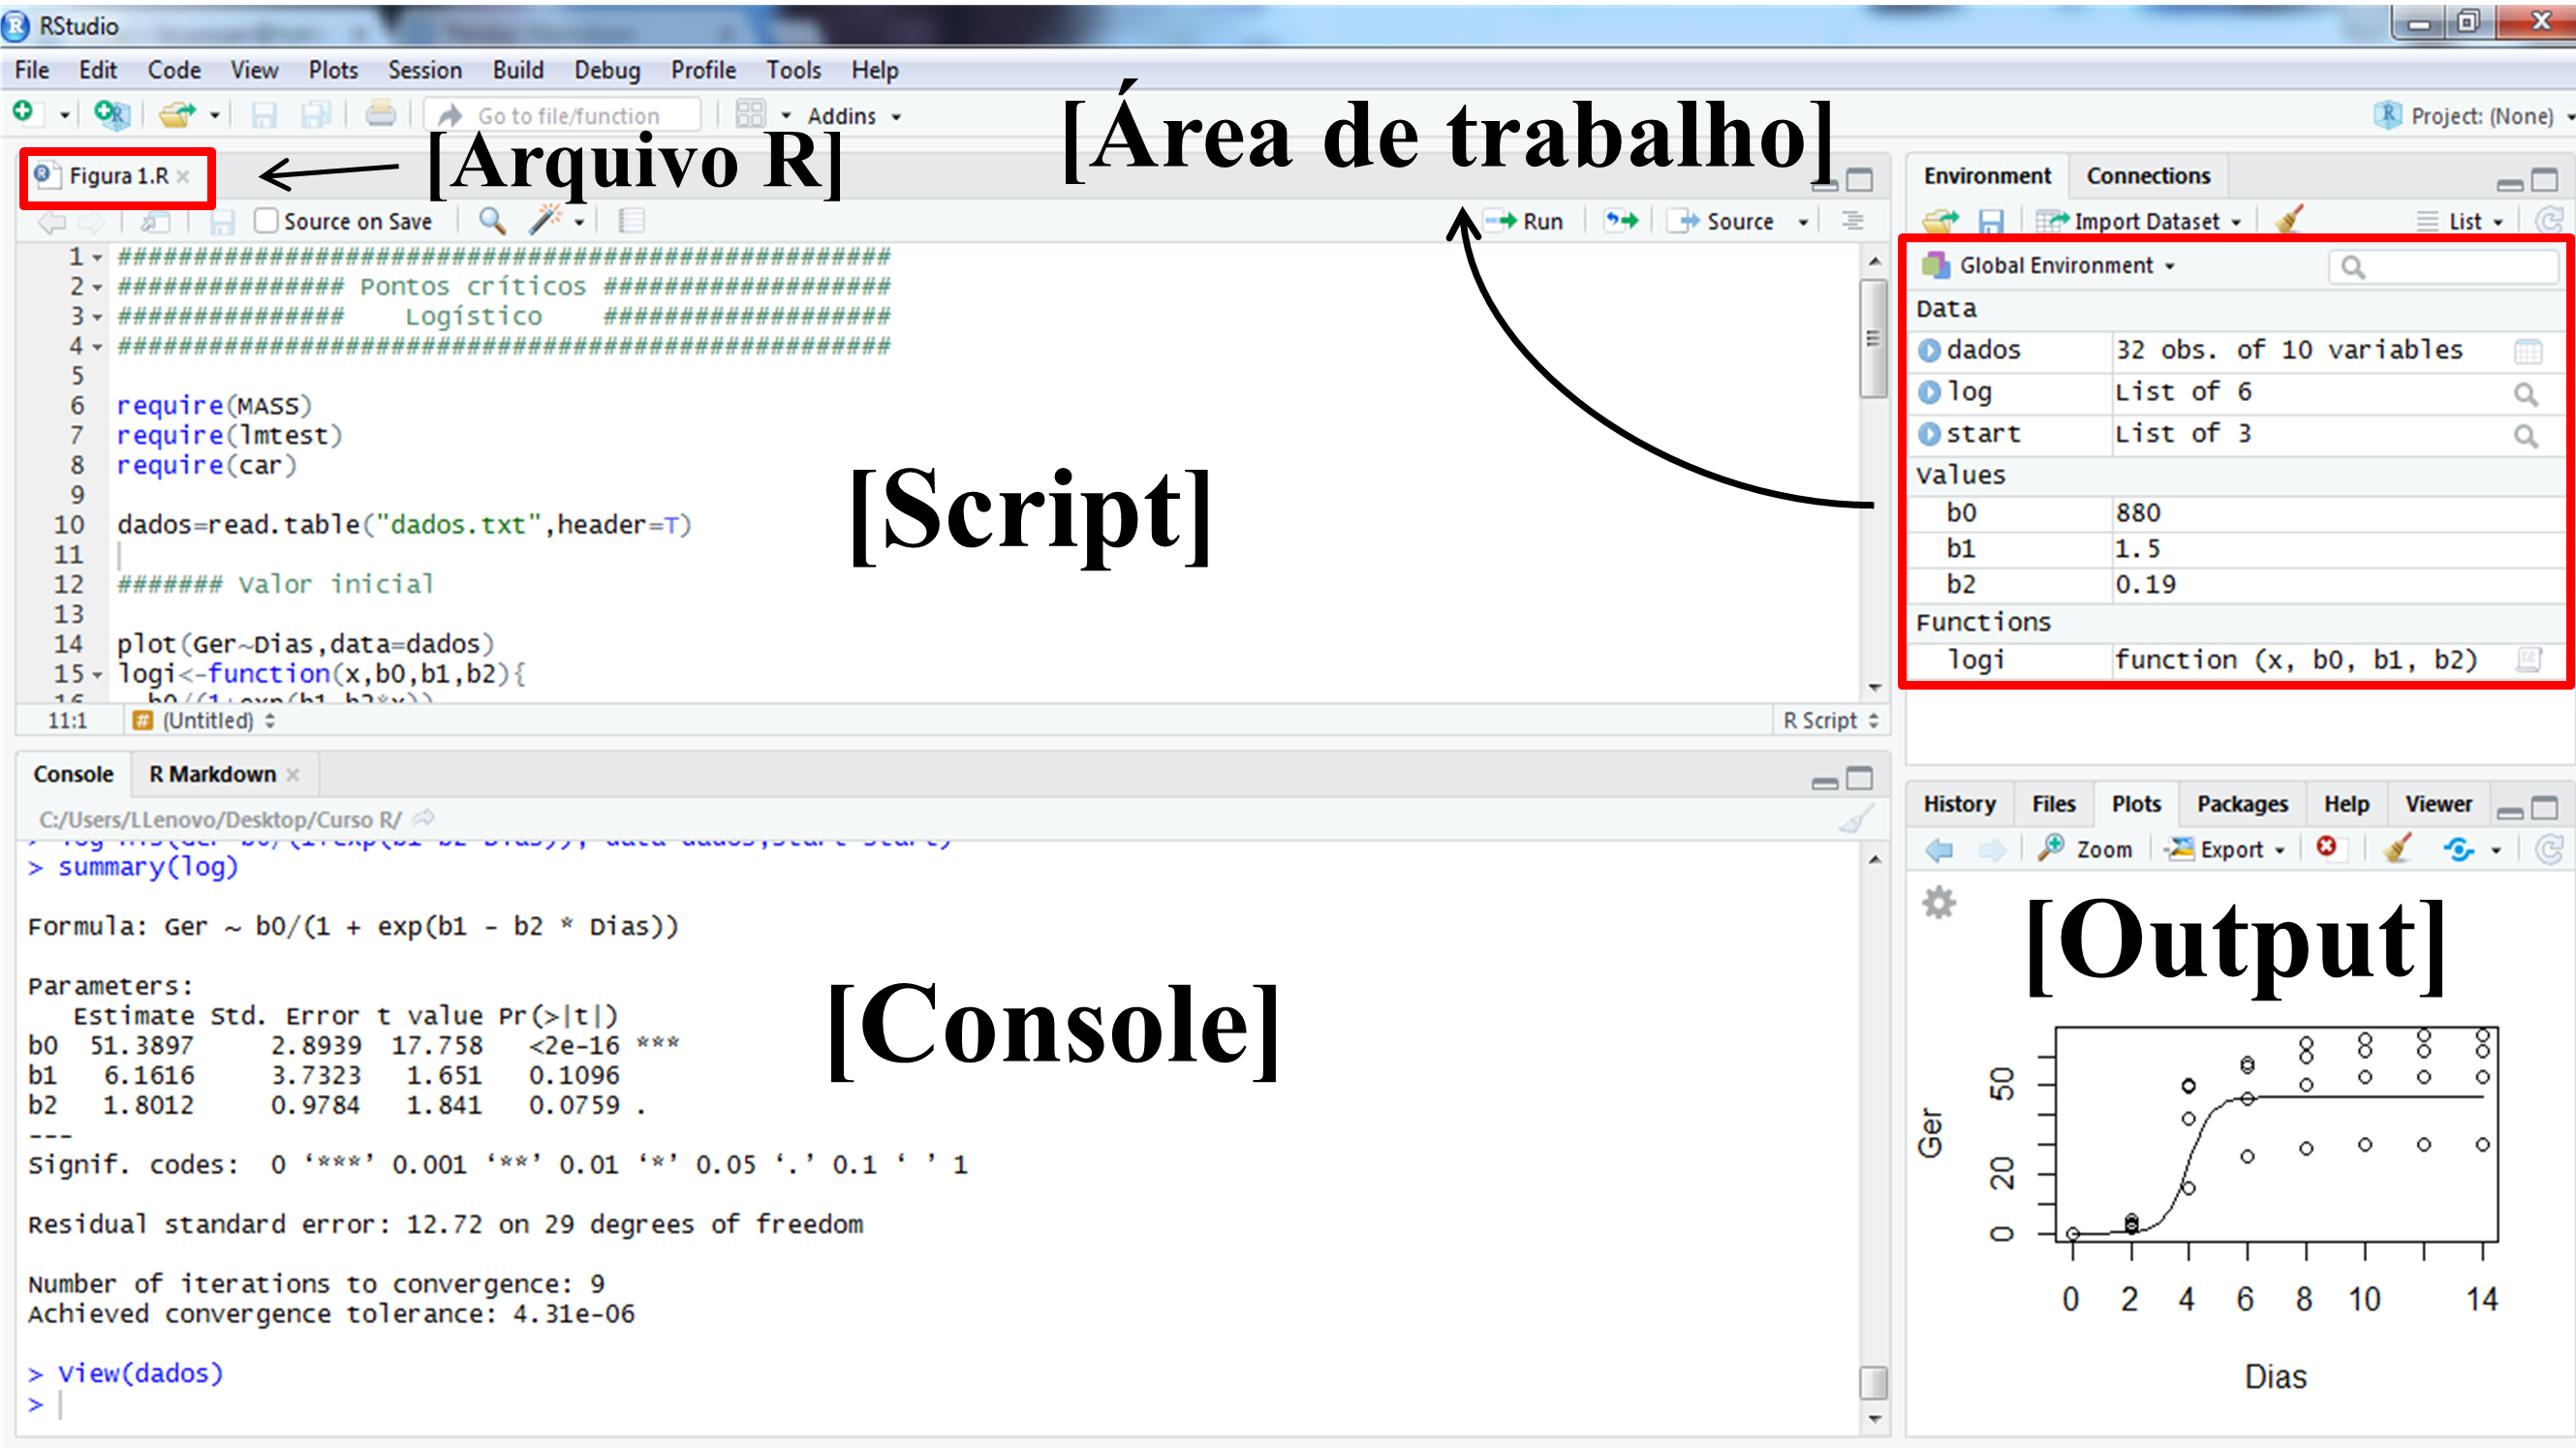
\includegraphics{figures/Console.png}
\caption{Interface do RStudio}
\end{figure}

Antes de iniciar as análises, recomenda-se escolher um diretório \indt{diretório} onde devem estar os \emph{inputs} (dados) e para onde serão enviados os \emph{outputs} (gráficos, arquivos .txt, .xlsx, etc) \indt{imputs}\indt{outputs}. Para selecionar o diretório, basta seguir o caminho \emph{Session \textgreater{} Set Working Directory \textgreater{} Choosing diretory} ou utilizar as teclas de atalho \emph{Ctrl+Shift+H}.

\begin{figure}
\centering
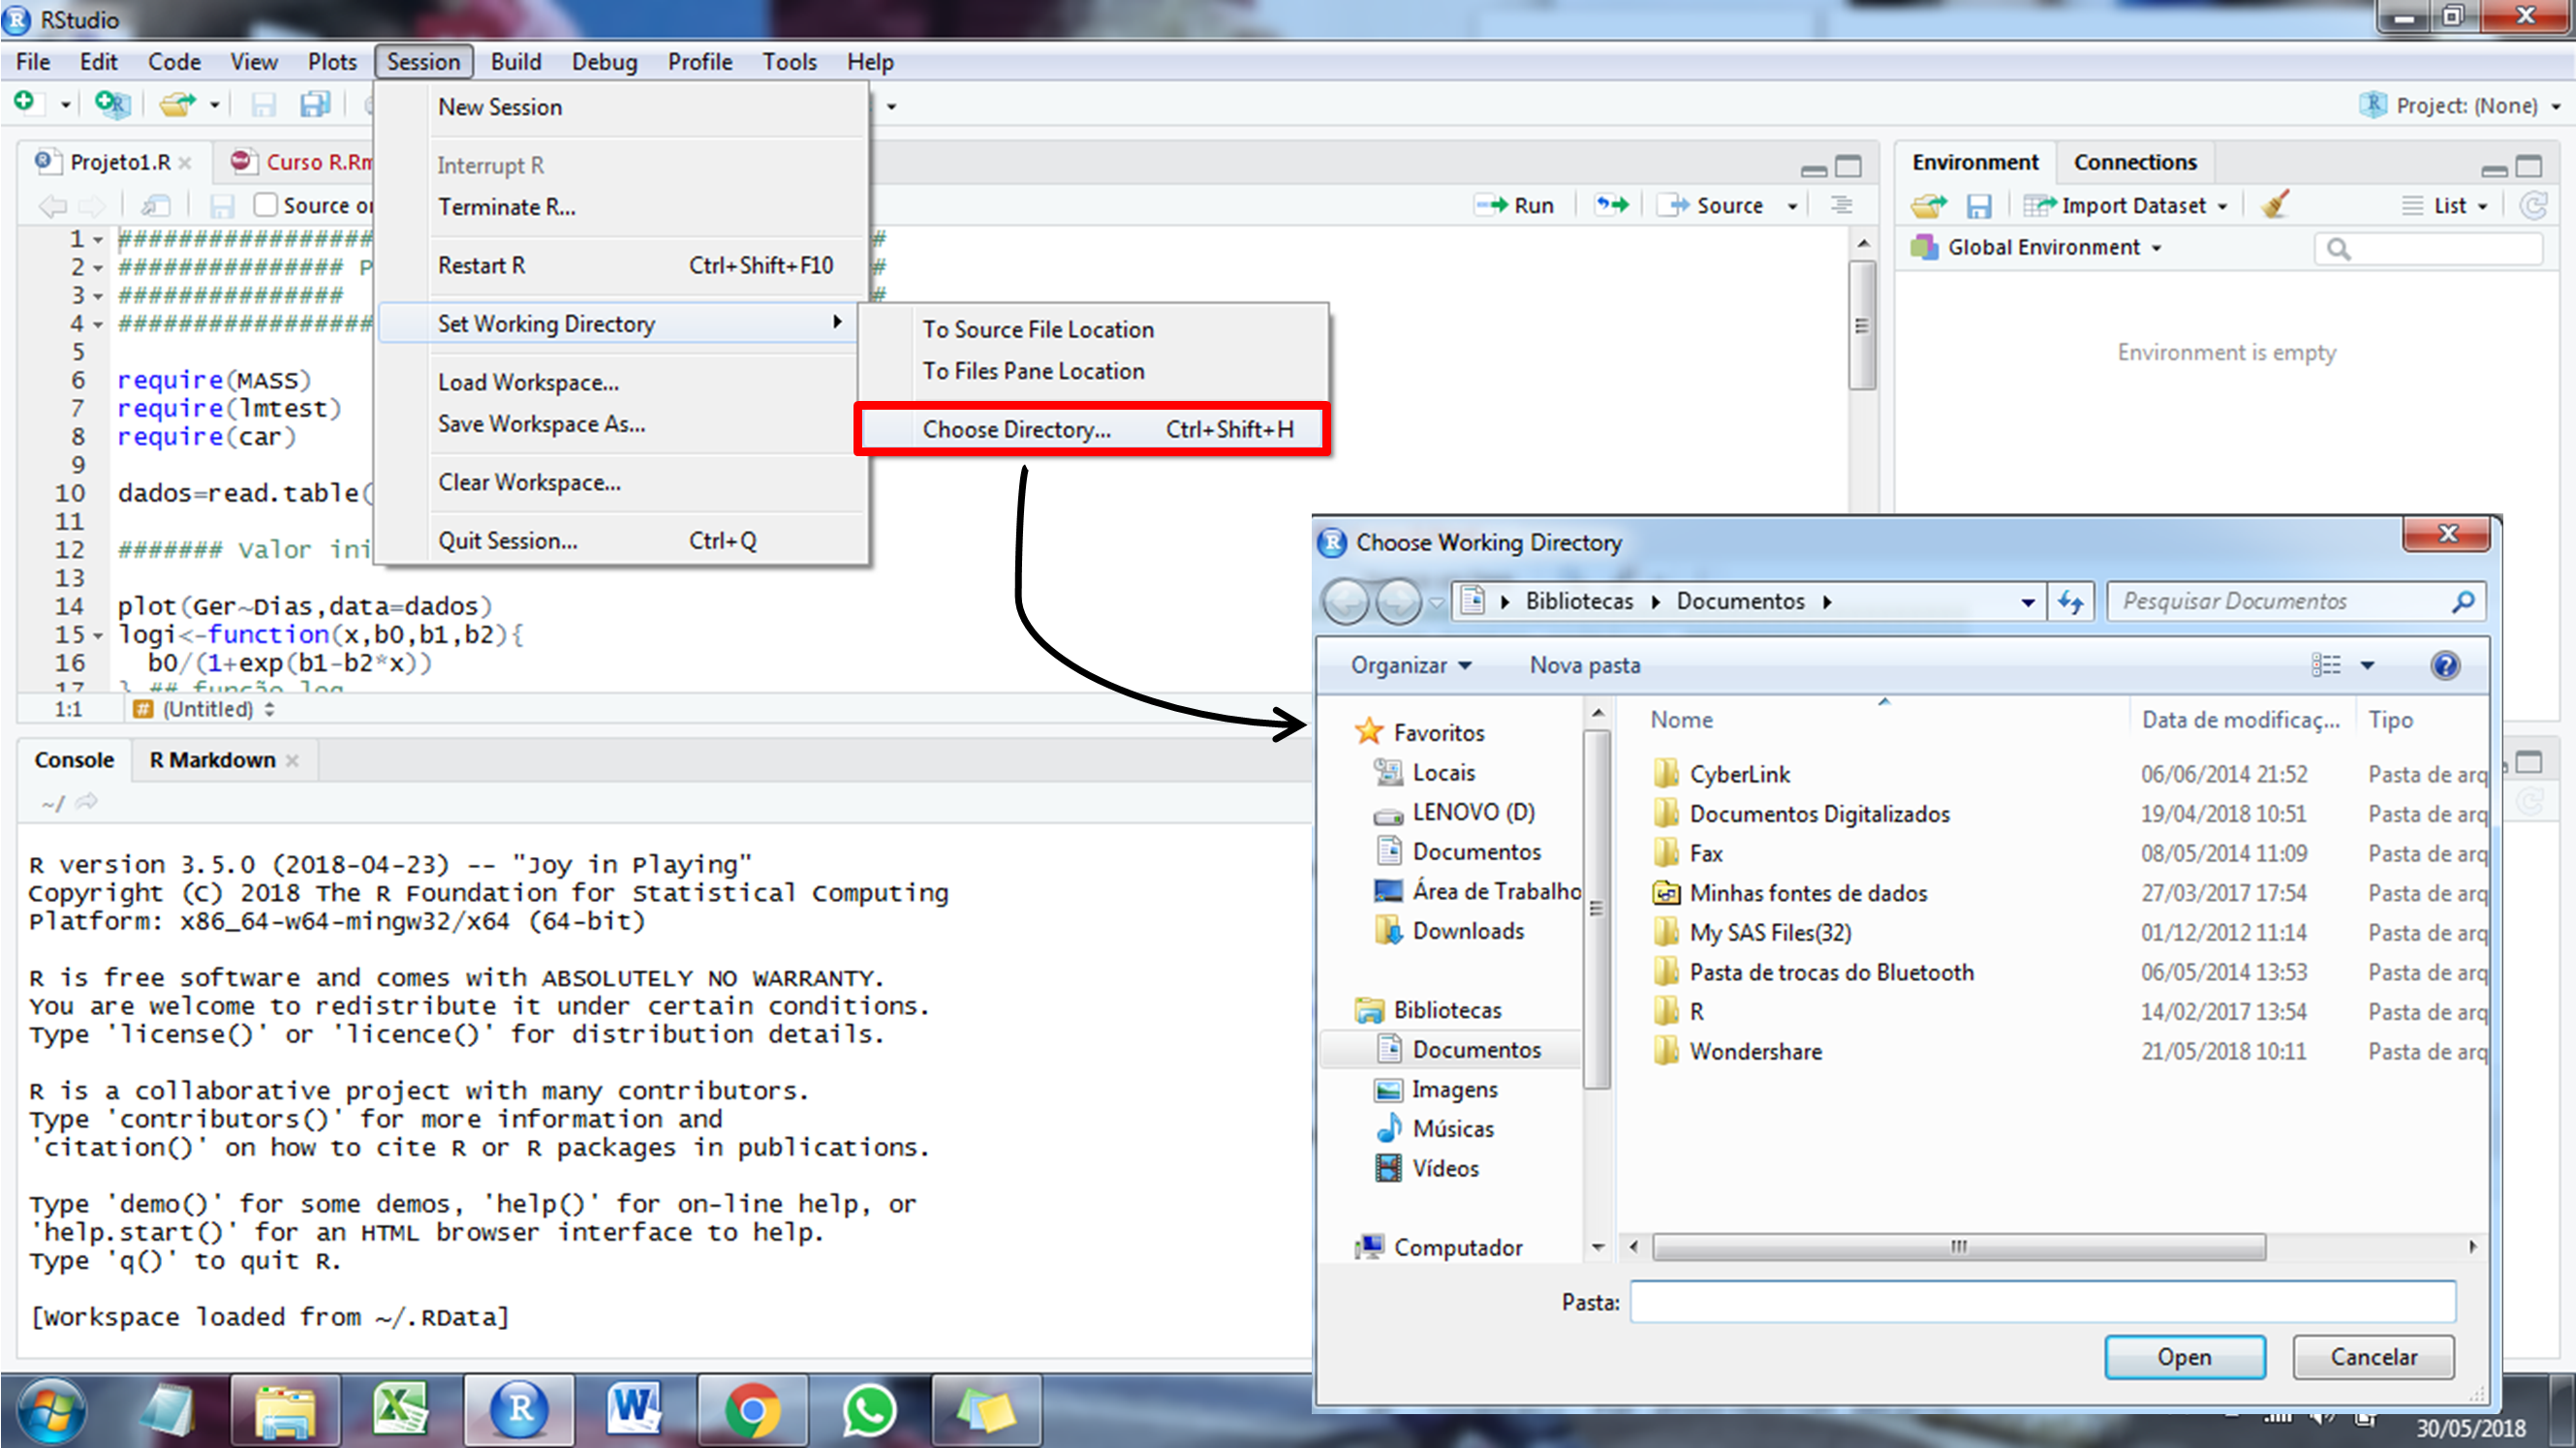
\includegraphics{figures/Diretory.png}
\caption{Selecionando um diretório}
\end{figure}

Posteriormente, um \emph{R Script} é iniciado conforme a figura abaixo ou pelas teclas de atalho \emph{Ctrl+Shift+N}. No canto inferior direito, além de servir como \emph{output} para gráficos (\emph{Plots}), também é o local onde os pacotes utilizados nas análises (\emph{Packages}) são instalados e maiores informações sobre as funções podem ser encontradas (\emph{Help}).

\hypertarget{meu-primeiro-script}{%
\section{Meu primeiro script}\label{meu-primeiro-script}}

Se você realizou o download do software R pela primeira vez e achou um tanto quanto ``estranho'' o pequeno tamanho do arquivo (\textasciitilde{}80 Mb), provalemente deve ter se perguntado como um software estatistico tão poderoso pode ser comprimido em um arquivo tão pequeno (pequeno em comparação com os +20 GB do SAS). A resposta é simples, somente os pacote básicos do R são baixados com o arquivo de instalação. Na medida em que o usuário necessita realizar uma análise específica, a instalação de um pacote que contém uma função específica para realizar tal análise é necessária.

A instalação dos pacotes pode ser realizada conforme a figura abaixo, ou através da função \texttt{install.packages()}. Após a instalação do pacote, o usuário deve utilizar as funções \texttt{require()} ou \texttt{library()} \indt{require} \indt{library}para que o pacote seja carregado e as suas funções possam ser utilizadas. Quando o usuário tenta utilizar uma função pertencente a um determinado pacote e este pacote não está instalado (ou carregado), um erro é exibido.

\begin{figure}
\centering
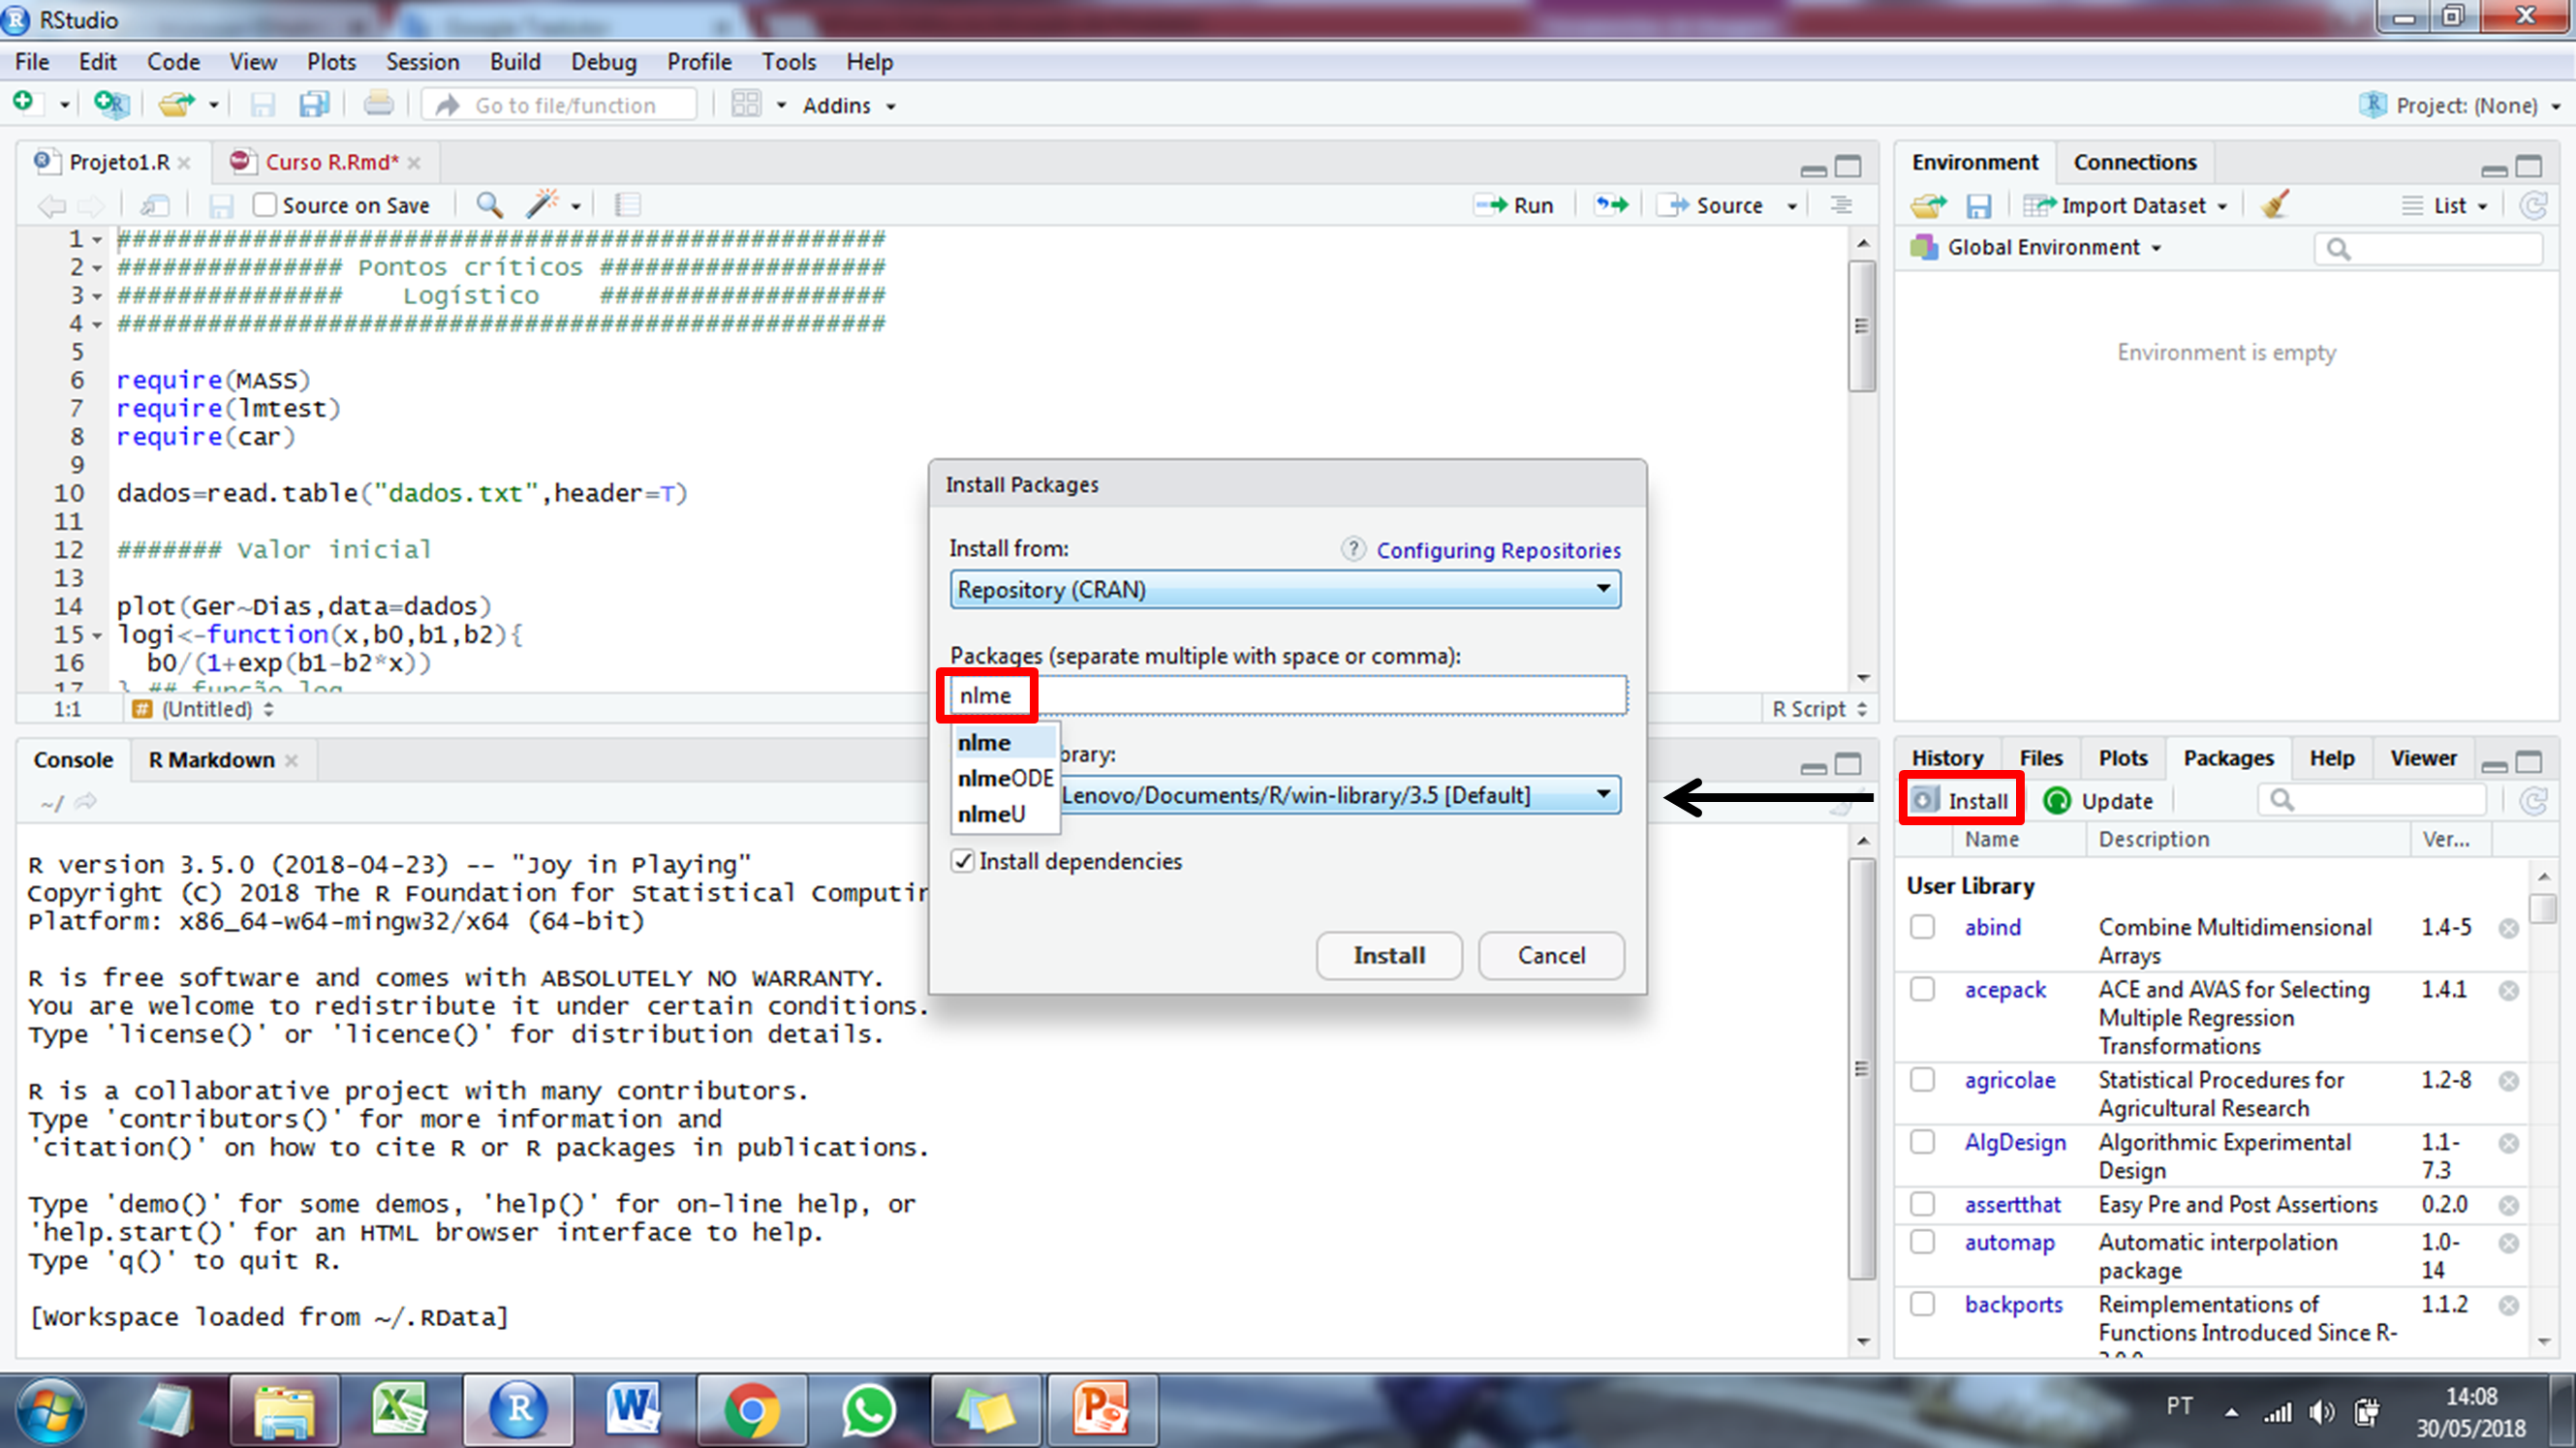
\includegraphics{figures/Install.png}
\caption{Instalando pacotes}
\end{figure}

\begin{figure}
\centering
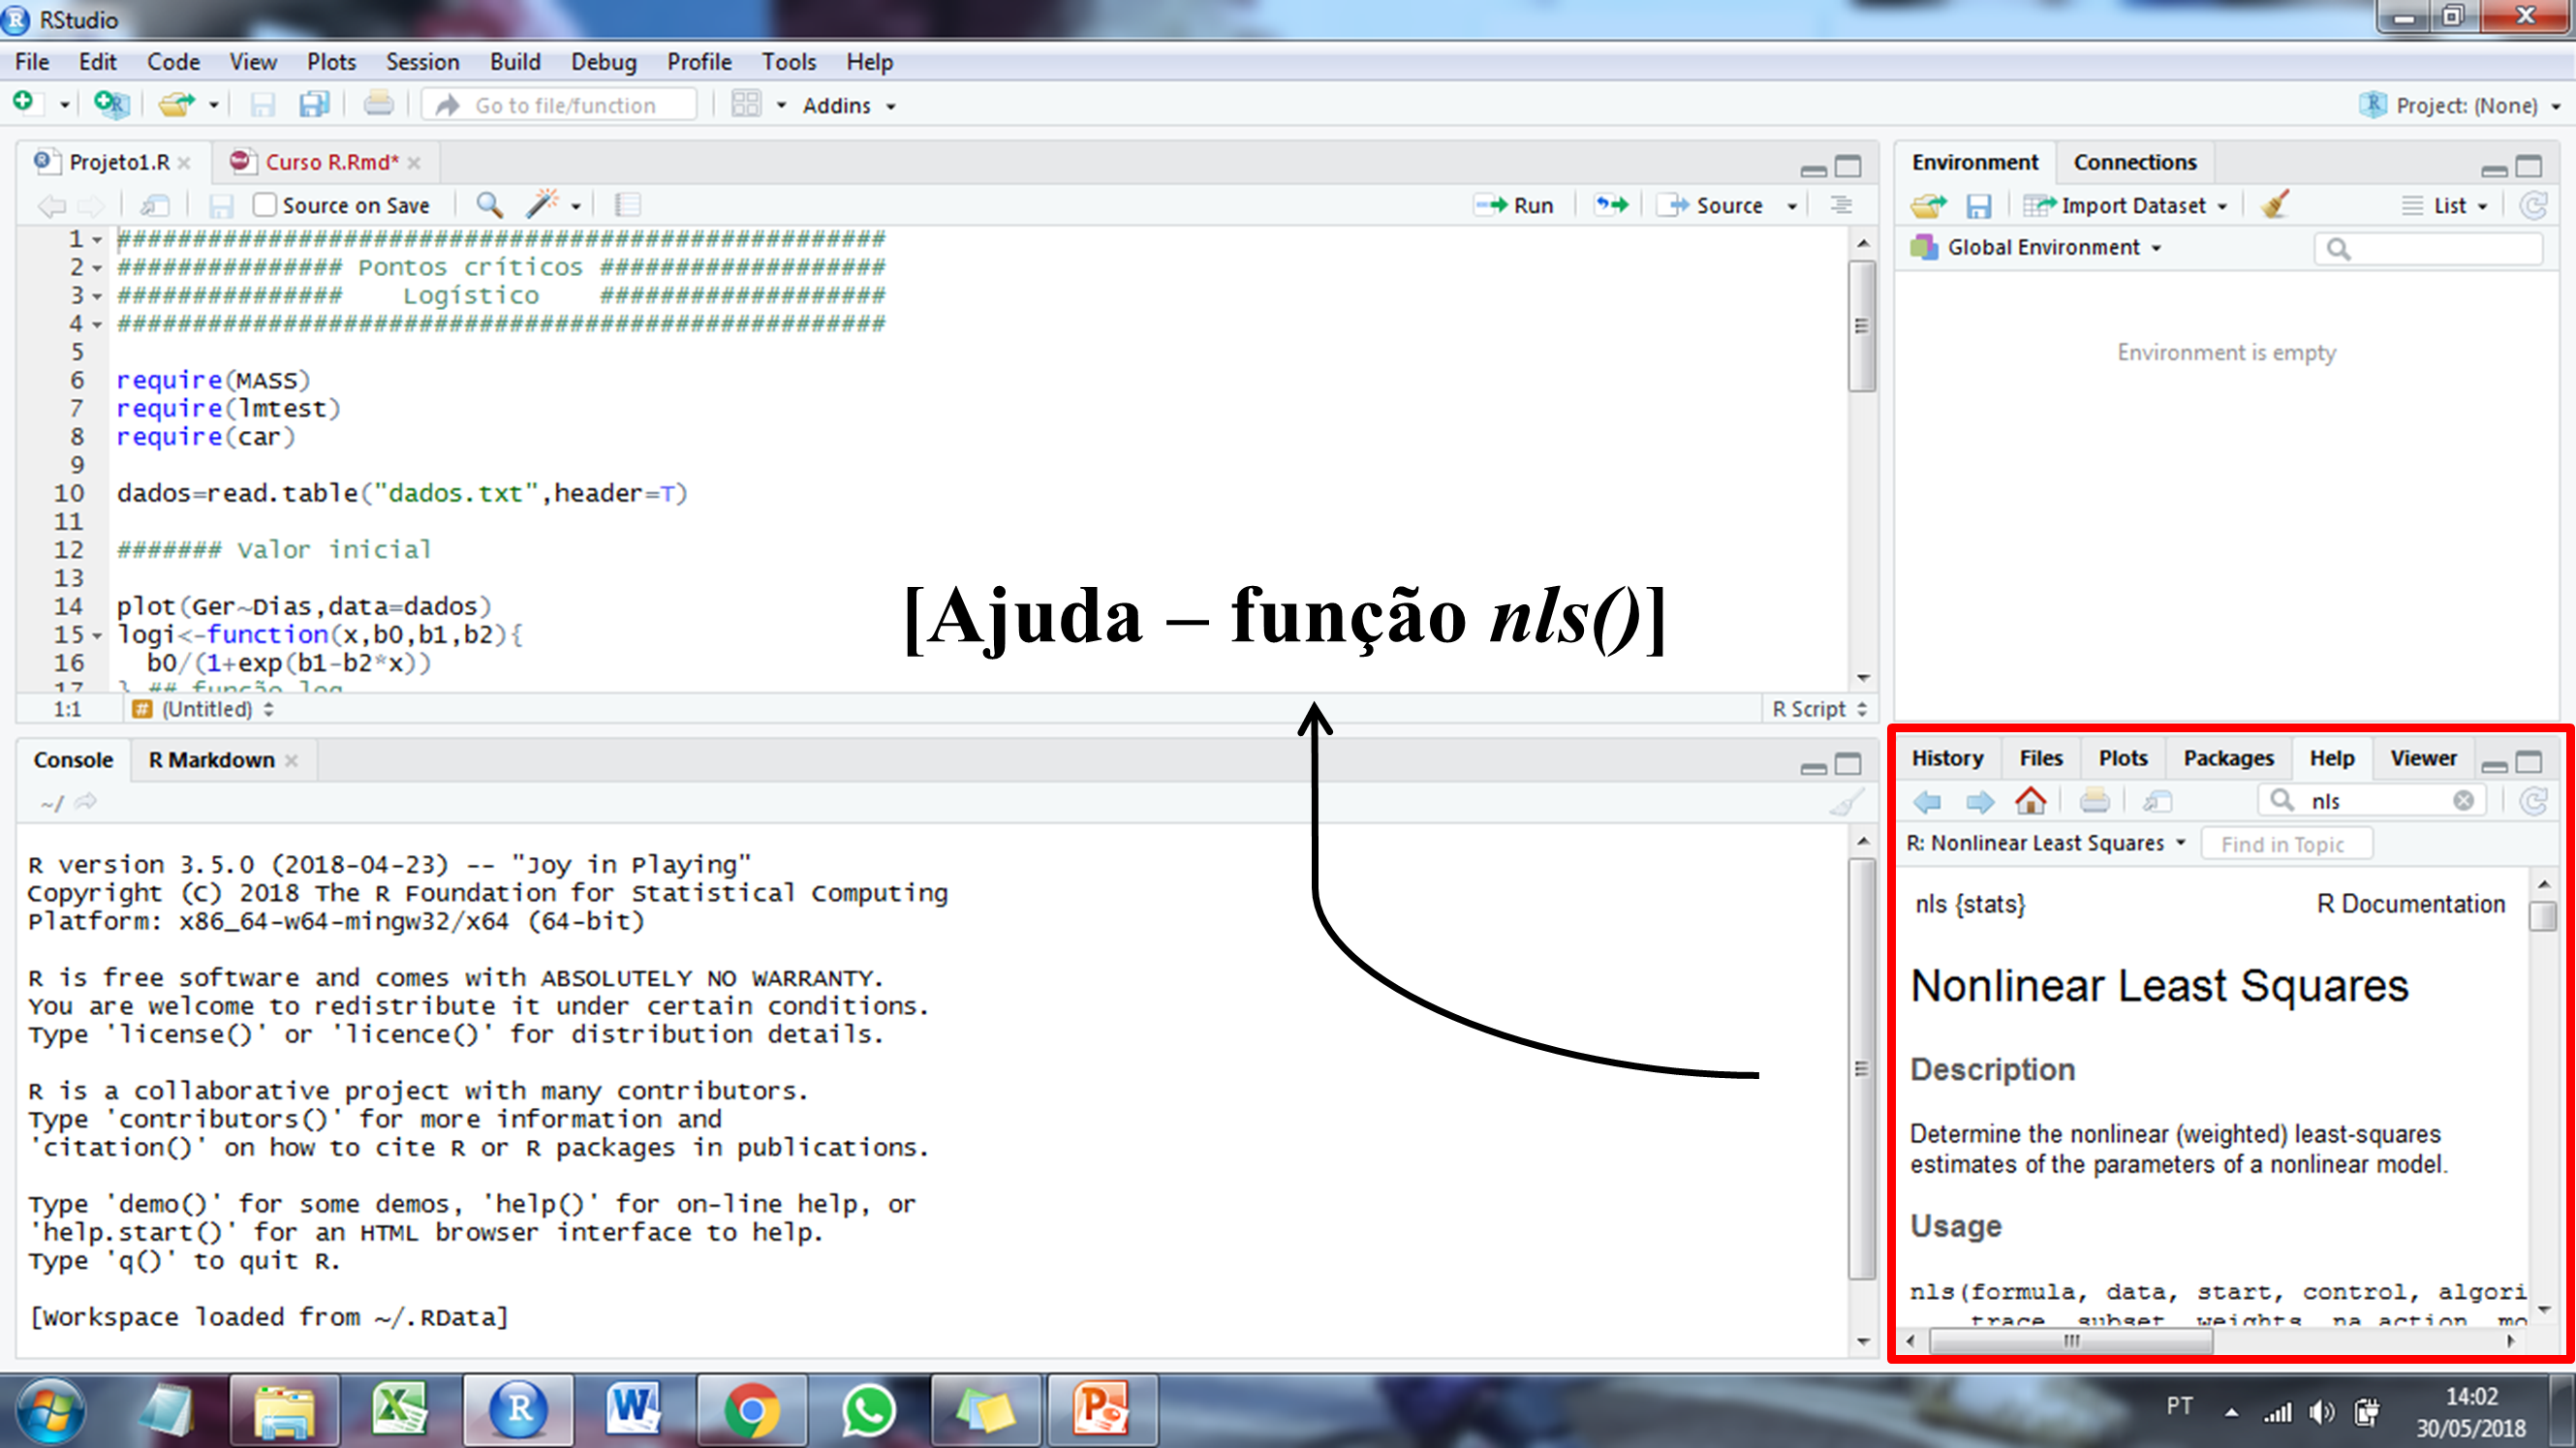
\includegraphics{figures/Help.png}
\caption{Ajuda para a função \texttt{nls()}}
\end{figure}

Como exemplo inicial, vamos tentar selecionar a variável \emph{Sepal.Length} do conjunto de dados base \texttt{iris} utilizando a função abaixo. \textbf{Cuidado, spoilers do pacote dplyr!} O primero passo é criar um novo script, seguindo os seguintes passos: \emph{File \textgreater{} New File \textgreater{} R script} ou utilizando o atalho \texttt{Ctrl+Shift+N}. Posteriormente, o seguinte código é digitado e executado ao se selecionar a linha do código e clicar no botão \emph{run} ou utilizando o atalho \texttt{Ctrl+Enter}).

\begin{Shaded}
\begin{Highlighting}[]
\NormalTok{SL =}\StringTok{ }\KeywordTok{select}\NormalTok{(iris, Sepal.Length)}
\end{Highlighting}
\end{Shaded}

\begin{verbatim}
Error in select(iris, Sepal.Length): unused argument (Sepal.Length)
\end{verbatim}

Neste caso, um erro é exibido pois o pacote \textbf{dplyr} não está instalado ou carregado. Caso ele já estiver instalado, a mensagem de erro acima é superada ao carregar o pacote antes de rodar a função.

\begin{Shaded}
\begin{Highlighting}[]
\KeywordTok{library}\NormalTok{(dplyr)}
\NormalTok{SL =}\StringTok{ }\KeywordTok{select}\NormalTok{(iris, Sepal.Length)}
\end{Highlighting}
\end{Shaded}

Caso o pacote \textbf{dplyr} não esteja instalado, a maneira mais fácil de instalá-lo é instalando a coleção de pacotes \href{https://www.tidyverse.org/}{tidyverse}\footnote{\url{https://www.tidyverse.org/}} seguindo os passos da Figura 3 ou utilizando a seguinte função.

\begin{Shaded}
\begin{Highlighting}[]
\KeywordTok{install.packages}\NormalTok{(}\StringTok{"tidyverse"}\NormalTok{, }\DataTypeTok{dependencies =} \OtherTok{TRUE}\NormalTok{)}
\KeywordTok{library}\NormalTok{(tidyverse)}
\end{Highlighting}
\end{Shaded}

O \textbf{tidyverse} é uma coleção de pacotes R projetados para a ciência de dados, contendo, dentre outros, seguintes pacotes que serão utilizados neste material.

\begin{itemize}
\tightlist
\item
  \textbf{ggplot2}, para criação de gráficos.
\item
  \textbf{dplyr}, para manipulação de dados.
\item
  \textbf{tidyr}, para organização de dados.
\item
  \textbf{tibble}, para criação de tibbles.
\end{itemize}

Praticamente todas as rotinas realizadas no R são baseadas em bibliotecas de códigos. Com a manipulaçao de pacotes não seria diferente. O pacote \href{https://github.com/trinker/pacman}{pacman}\footnote{\url{https://github.com/trinker/pacman}} é uma ferramenta de gerenciamento de pacotes R que combina a funcionalidade das funções relacionadas à biblioteca base em funções intuitivamente nomeadas, reduzindo o código para executar simultaneamente várias ações. Uma das funções mais úteis do pacote pacman é a \texttt{p\_load()}\indf{p\_load} (\emph{package load}). Esta função checa se um pacote está instalado e em caso afirmativo, carrega-o como se a função \texttt{library()} tivesse sido usada. Caso o pacote não esteja instalado, ela primeiro o instala-rá antes de carregá-lo. Vamos, agora, instalar (para quem está utilizando o R pela primeira vez) ou carregar (para quem já tem instalado) os pacotes utilizados neste material.

\begin{Shaded}
\begin{Highlighting}[]
\ControlFlowTok{if}\NormalTok{ (}\OperatorTok{!}\KeywordTok{require}\NormalTok{(}\StringTok{"pacman"}\NormalTok{)) }\KeywordTok{install.packages}\NormalTok{(}\StringTok{"pacman"}\NormalTok{)}
\KeywordTok{library}\NormalTok{(pacman)}
\KeywordTok{p_load}\NormalTok{(hnp, asbio, car, dplyr, emmeans, effects, multcomp, lme4, readxl,}
\NormalTok{       ExpDes, manipulate, cowplot, tidyverse, agricolae, psych, corrplot,}
\NormalTok{       pvclust, factoextra, kableExtra, ggfortify)}

\KeywordTok{p_load_gh}\NormalTok{(}\StringTok{"TiagoOlivoto/metan"}\NormalTok{)}
\end{Highlighting}
\end{Shaded}

Os pacotes disponibilizados no software \emph{R} estão em constante atualização. Utilizando a função \texttt{packageStatus()} e \texttt{summary(packageStatus())} é possível verificar se os pacotes estão atualizados. Outra forma é ir em \emph{Packages \textgreater{} Update} que se encontra no canto inferior direito conforme demonstrado na Figura 5. Por fim, para citar os pacotes \indt{pacotes}, recomenda-se verificar a referência através da função \texttt{citation()}. \indt{citação de pacotes} \indt{atualização}

\begin{figure}
\centering
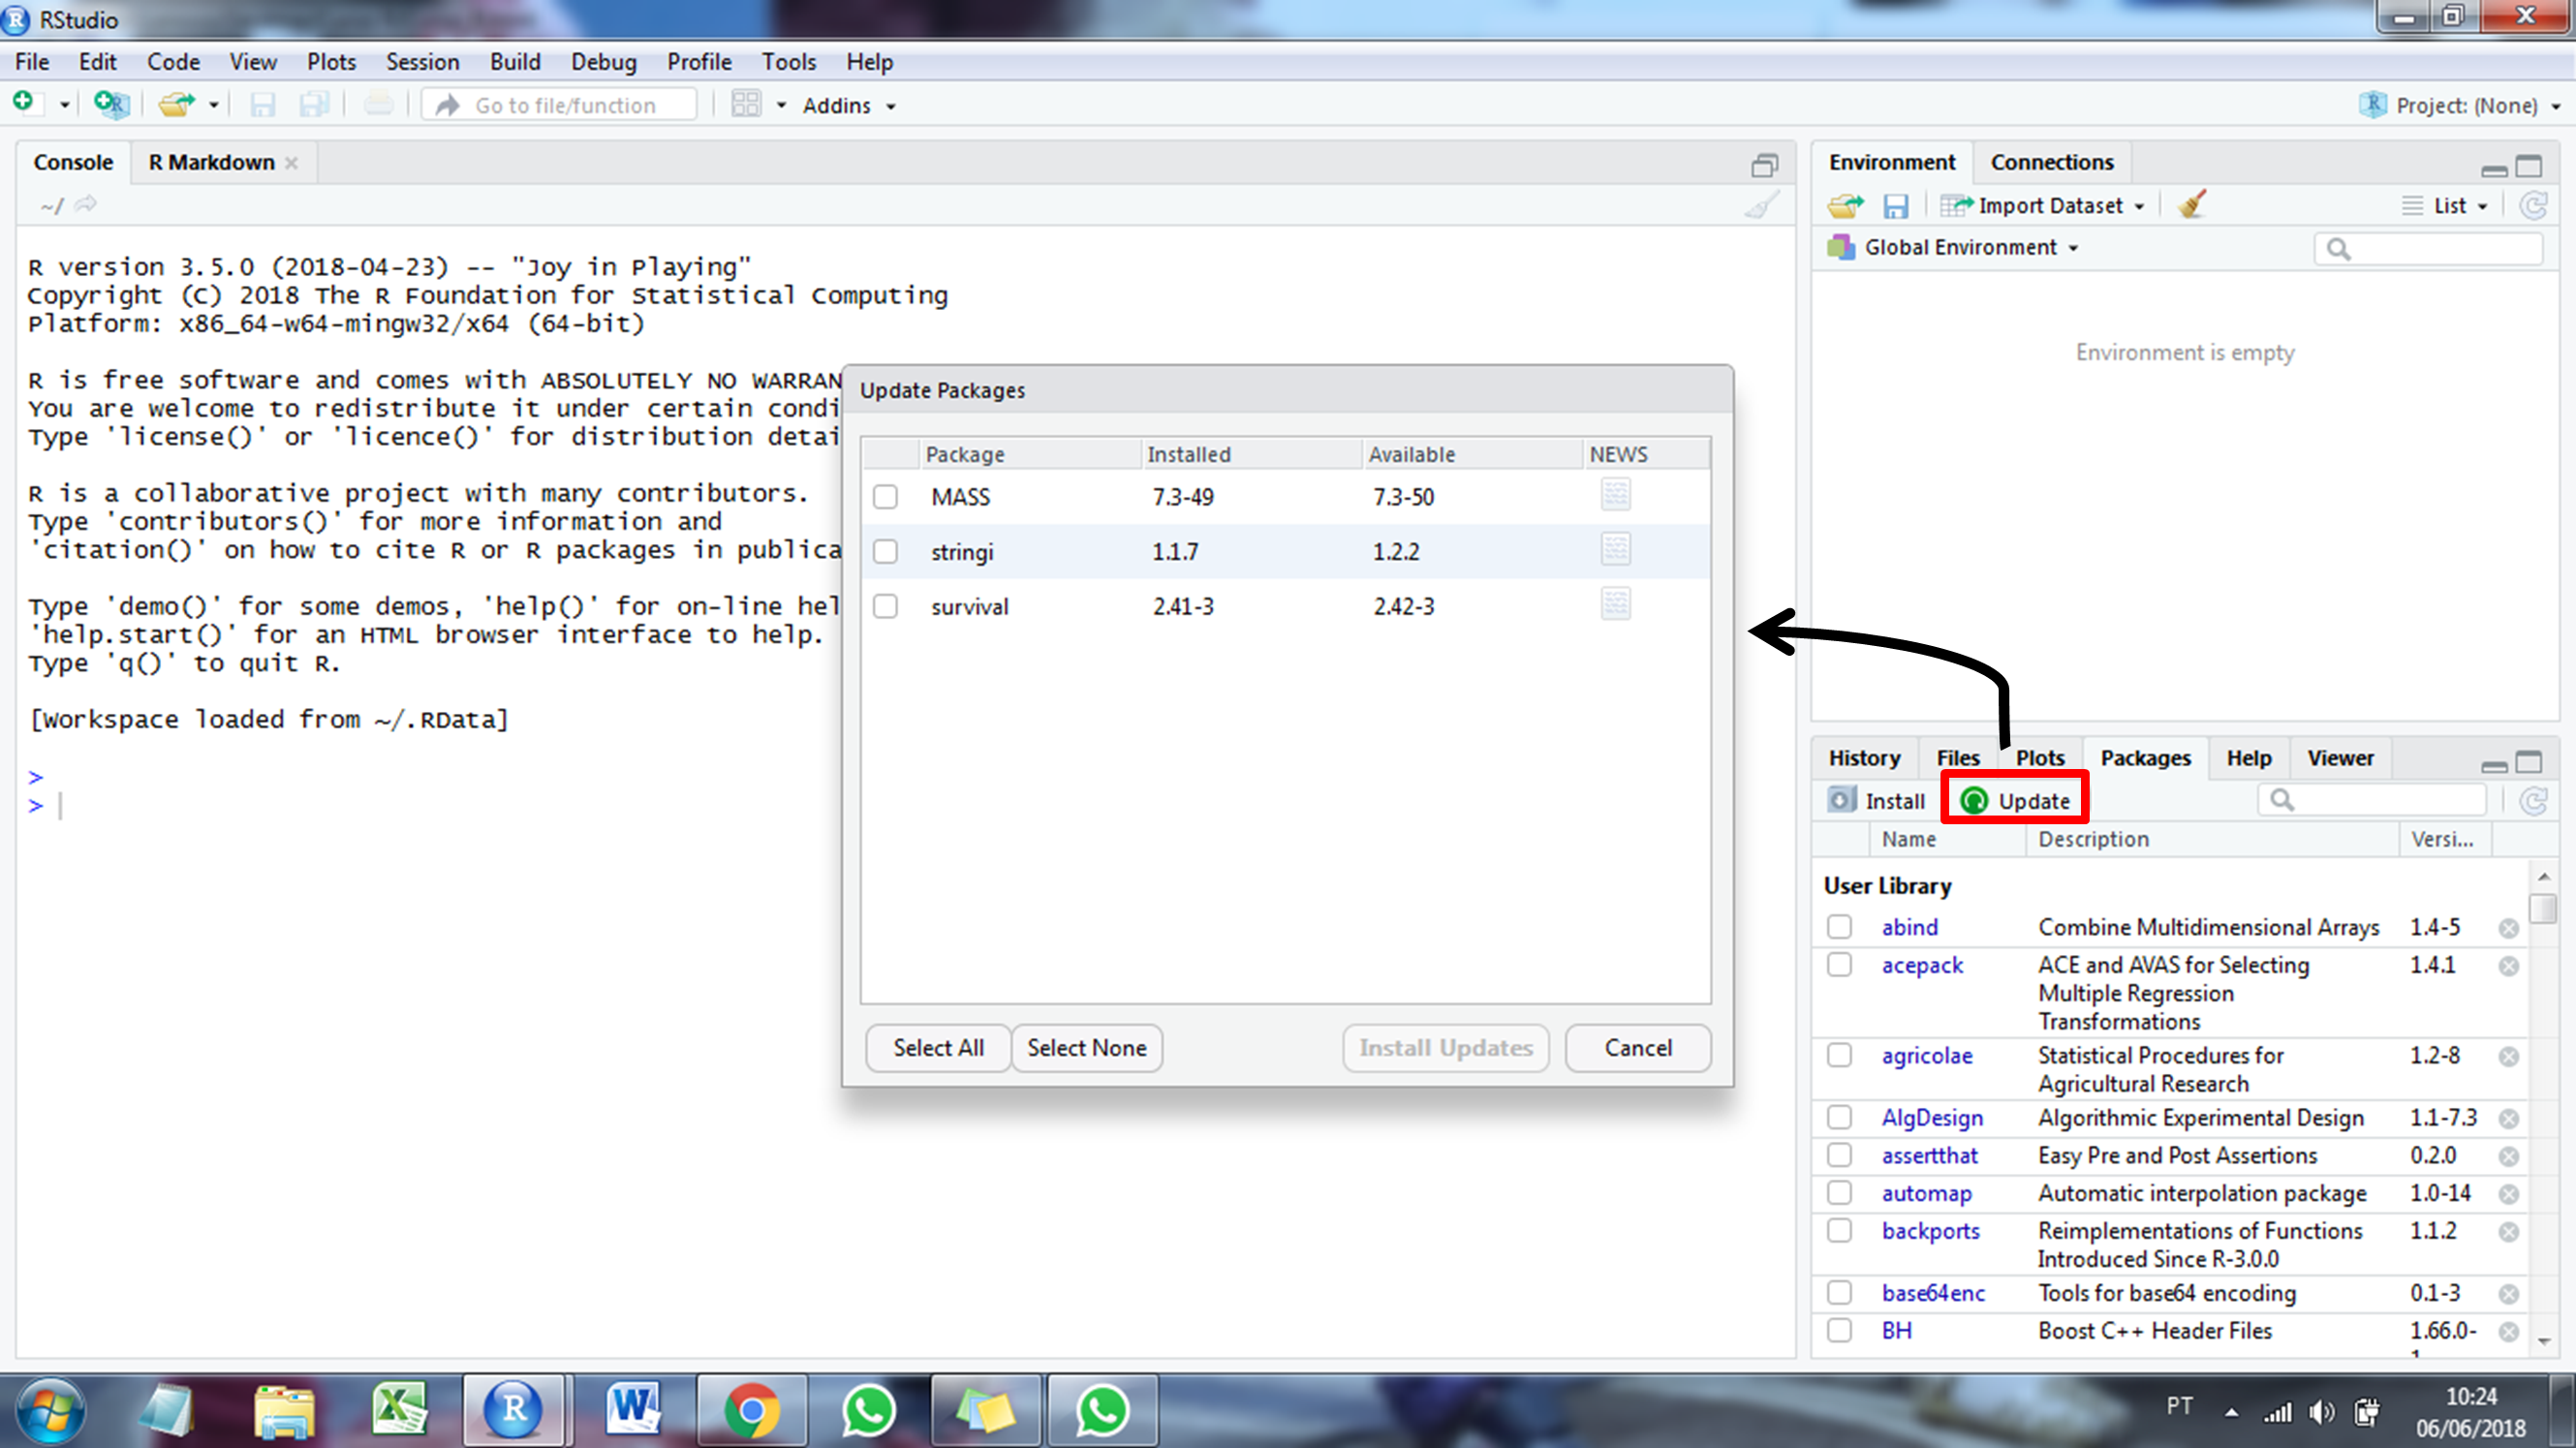
\includegraphics{figures/Update.png}
\caption{Verificando se há atualizações disponíveis}
\end{figure}

\begin{Shaded}
\begin{Highlighting}[]
\KeywordTok{citation}\NormalTok{(}\StringTok{"dplyr"}\NormalTok{)}
\end{Highlighting}
\end{Shaded}

\begin{verbatim}

To cite package 'dplyr' in publications use:

  Hadley Wickham, Romain François, Lionel Henry and Kirill Müller
  (2019). dplyr: A Grammar of Data Manipulation. R package version
  0.8.3. https://CRAN.R-project.org/package=dplyr

A BibTeX entry for LaTeX users is

  @Manual{,
    title = {dplyr: A Grammar of Data Manipulation},
    author = {Hadley Wickham and Romain François and Lionel Henry and Kirill Müller},
    year = {2019},
    note = {R package version 0.8.3},
    url = {https://CRAN.R-project.org/package=dplyr},
  }
\end{verbatim}

\hypertarget{objects}{%
\chapter{Tipos de objetos}\label{objects}}

Os tipos de objeto mais utilizados na linguagem \emph{R} são: (i) vetores, (ii) matrizes, (iii) data frames, (iv) listas e (v) funções. Um enfoque maior será dado aos vetores, matrizes e data frames, pois estes são amplamente utilizados, inclusive nas análises mais simples.

\hypertarget{vetores}{%
\section{Vetores}\label{vetores}}

A função \texttt{c()} \indt{vetores} \indf{c} combina valores que formam vetores\footnote{Vetores são uma estrutura de dados básica do R que permite armazenar um conjunto de valores numéricos ou de caracteres em um objeto nomeado}. Abaixo, é demonstrado como vetores podem ser criados utilizando \texttt{c()}.

\begin{Shaded}
\begin{Highlighting}[]
\NormalTok{x1 =}\StringTok{ }\KeywordTok{c}\NormalTok{(}\DecValTok{1}\NormalTok{) }\CommentTok{# Escalar }
\NormalTok{x2 =}\StringTok{ }\KeywordTok{c}\NormalTok{(}\DecValTok{1}\NormalTok{,}\DecValTok{2}\NormalTok{) }\CommentTok{# Vetor}
\NormalTok{x3 =}\StringTok{ }\KeywordTok{c}\NormalTok{(}\DecValTok{1}\NormalTok{,}\DecValTok{2}\NormalTok{,}\DecValTok{3}\NormalTok{) }\CommentTok{# Vetor}
\NormalTok{x3}
\end{Highlighting}
\end{Shaded}

\begin{verbatim}
[1] 1 2 3
\end{verbatim}

\begin{Shaded}
\begin{Highlighting}[]
\NormalTok{x3}\FloatTok{.1}\NormalTok{ =}\StringTok{ }\KeywordTok{c}\NormalTok{(}\StringTok{"um"}\NormalTok{,}\StringTok{"dois"}\NormalTok{,}\StringTok{"três") # Vetor com caracteres}
\end{Highlighting}
\end{Shaded}

Os vetores foram armazenados em \emph{x1}, \emph{x2} e \emph{x3} e ficaram armazenados como valores na área de trabalho como valores (\emph{values}). Para que os valores sejam mostrados basta digitar no \emph{console} onde os vetores foram armazenados.

Vetores também podem ser criados utilizando as funções \texttt{rep()} e \texttt{seq()}, conforme mostrado abaixo. \indf{rep} \indf{seq}

\begin{Shaded}
\begin{Highlighting}[]
\KeywordTok{rep}\NormalTok{(}\DecValTok{5}\NormalTok{, }\DecValTok{10}\NormalTok{)}
\end{Highlighting}
\end{Shaded}

\begin{verbatim}
 [1] 5 5 5 5 5 5 5 5 5 5
\end{verbatim}

\begin{Shaded}
\begin{Highlighting}[]
\KeywordTok{seq}\NormalTok{(}\DecValTok{1}\NormalTok{, }\DecValTok{5}\NormalTok{)}
\end{Highlighting}
\end{Shaded}

\begin{verbatim}
[1] 1 2 3 4 5
\end{verbatim}

\begin{Shaded}
\begin{Highlighting}[]
\KeywordTok{seq}\NormalTok{(}\DecValTok{1}\NormalTok{, }\DecValTok{5}\NormalTok{, }\DataTypeTok{by =} \FloatTok{0.5}\NormalTok{)}
\end{Highlighting}
\end{Shaded}

\begin{verbatim}
[1] 1.0 1.5 2.0 2.5 3.0 3.5 4.0 4.5 5.0
\end{verbatim}

\begin{Shaded}
\begin{Highlighting}[]
\KeywordTok{seq}\NormalTok{(}\DecValTok{2}\NormalTok{, }\DecValTok{20}\NormalTok{, }\DataTypeTok{by =} \DecValTok{2}\NormalTok{)}
\end{Highlighting}
\end{Shaded}

\begin{verbatim}
 [1]  2  4  6  8 10 12 14 16 18 20
\end{verbatim}

A função \texttt{c()} também pode ser combinada com as funções \texttt{rep()} e \texttt{seq()} para criar vetores mais complexos, como mostrado abaixo.

\begin{Shaded}
\begin{Highlighting}[]
\NormalTok{x4 =}\StringTok{ }\KeywordTok{c}\NormalTok{(}\KeywordTok{rep}\NormalTok{(}\DecValTok{1}\OperatorTok{:}\DecValTok{4}\NormalTok{, }\DataTypeTok{each =} \DecValTok{4}\NormalTok{))}
\NormalTok{x5 =}\StringTok{ }\KeywordTok{seq}\NormalTok{(}\DecValTok{1}\OperatorTok{:}\DecValTok{5}\NormalTok{)}
\NormalTok{x6 =}\StringTok{ }\KeywordTok{c}\NormalTok{(}\KeywordTok{rep}\NormalTok{(}\KeywordTok{seq}\NormalTok{(}\DecValTok{1}\OperatorTok{:}\DecValTok{5}\NormalTok{), }\DataTypeTok{each =} \DecValTok{2}\NormalTok{))}
\NormalTok{x6}
\end{Highlighting}
\end{Shaded}

\begin{verbatim}
 [1] 1 1 2 2 3 3 4 4 5 5
\end{verbatim}

Utilizando colchtes {[} {]} é possível selecionar um (ou um conjunto) de elementos de um vetor. Por exemplo:

\begin{Shaded}
\begin{Highlighting}[]
\NormalTok{x7 =}\StringTok{ }\NormalTok{x6[}\DecValTok{1}\NormalTok{] }\CommentTok{# Seleciona o primeiro elemento do vetor }
\NormalTok{x8 =}\StringTok{ }\NormalTok{x6[}\DecValTok{4}\NormalTok{] }\CommentTok{#  Seleciona o quarto elemento do vetor }
\NormalTok{x9 =}\StringTok{ }\NormalTok{x6[}\KeywordTok{c}\NormalTok{(}\DecValTok{1}\NormalTok{, }\DecValTok{4}\NormalTok{, }\DecValTok{8}\NormalTok{)] }\CommentTok{# Seleciona o primeiro, o quarto e o oitavo elemento}
\NormalTok{x9}
\end{Highlighting}
\end{Shaded}

\begin{verbatim}
[1] 1 2 4
\end{verbatim}

\begin{Shaded}
\begin{Highlighting}[]
\NormalTok{x10 =}\StringTok{ }\NormalTok{x6[}\DecValTok{1}\OperatorTok{:}\DecValTok{4}\NormalTok{] }\CommentTok{# armazena uma sequência de elementos (primeiro ao quarto)}
\end{Highlighting}
\end{Shaded}

\hypertarget{matrizes}{%
\section{Matrizes}\label{matrizes}}

As matrizes \indt{matrizes} são um conjunto de valores (ou variáveis) dispostos em linhas e colunas, e que formam um corpo delimitado por {[} {]}. As matrizes são geralmente representadas genericamente por \({{\bm{A}}_{{\bm{MxN}}}}\), onde \textbf{M} e \textbf{N} represetam os números de linhas e colunas da matriz, respectivamente. As matrizes podem ser facilmente construídas utilizando a função \texttt{matrix()}. Alternativamente, as funções \texttt{cbind()} e \texttt{rbind()} também podem ser utilizadas. A primeira função adiciona colunas as matrizes, enquanto que a segunda adiciona linhas. Veremos mais tarde que estas funções podem ser combinadas com outras funções para construção de data frames \indf{data.frame}.

\begin{Shaded}
\begin{Highlighting}[]
\CommentTok{## Usando cbind()}
\NormalTok{x10 =}\StringTok{ }\KeywordTok{cbind}\NormalTok{(}\DecValTok{1}\NormalTok{,}\DecValTok{2}\NormalTok{,}\DecValTok{3}\NormalTok{,}\DecValTok{4}\NormalTok{,}\DecValTok{5}\NormalTok{) }\CommentTok{# ou x10 = cbind(1:5), 5 colunas com 1 elemento cada}
\NormalTok{x11 =}\StringTok{ }\KeywordTok{cbind}\NormalTok{(}\KeywordTok{c}\NormalTok{(}\DecValTok{1}\NormalTok{,}\DecValTok{2}\NormalTok{,}\DecValTok{3}\NormalTok{,}\DecValTok{4}\NormalTok{,}\DecValTok{5}\NormalTok{)) }\CommentTok{# ou x11 = cbind(c(1:5)), 1 coluna com 5 elementos cada }
\NormalTok{x12 =}\StringTok{ }\KeywordTok{cbind}\NormalTok{(}\KeywordTok{c}\NormalTok{(}\DecValTok{1}\NormalTok{,}\DecValTok{2}\NormalTok{,}\DecValTok{3}\NormalTok{,}\DecValTok{4}\NormalTok{,}\DecValTok{5}\NormalTok{),}\KeywordTok{c}\NormalTok{(}\DecValTok{6}\NormalTok{,}\DecValTok{7}\NormalTok{,}\DecValTok{8}\NormalTok{,}\DecValTok{9}\NormalTok{,}\DecValTok{10}\NormalTok{)) }\CommentTok{# 2 colunas de 5 elementos}
\NormalTok{x12}\FloatTok{.1}\NormalTok{ =}\StringTok{ }\KeywordTok{cbind}\NormalTok{(x11,}\KeywordTok{c}\NormalTok{(}\DecValTok{6}\OperatorTok{:}\DecValTok{10}\NormalTok{))}
\NormalTok{x13 =}\StringTok{ }\KeywordTok{cbind}\NormalTok{(}\KeywordTok{c}\NormalTok{(}\DecValTok{1}\NormalTok{,}\DecValTok{2}\NormalTok{,}\DecValTok{3}\NormalTok{,}\DecValTok{4}\NormalTok{,}\DecValTok{5}\NormalTok{),}\KeywordTok{c}\NormalTok{(}\DecValTok{6}\NormalTok{,}\DecValTok{7}\NormalTok{,}\DecValTok{8}\NormalTok{,}\DecValTok{9}\NormalTok{,}\DecValTok{10}\NormalTok{),}\KeywordTok{c}\NormalTok{(}\DecValTok{11}\NormalTok{,}\DecValTok{12}\NormalTok{,}\DecValTok{13}\NormalTok{,}\DecValTok{14}\NormalTok{,}\DecValTok{15}\NormalTok{)) }\CommentTok{# 3 colunas de 5 elementos}
\NormalTok{x13}\FloatTok{.1}\NormalTok{ =}\StringTok{ }\KeywordTok{cbind}\NormalTok{(x12}\FloatTok{.1}\NormalTok{,}\KeywordTok{c}\NormalTok{(}\DecValTok{11}\NormalTok{,}\DecValTok{12}\NormalTok{,}\DecValTok{13}\NormalTok{,}\DecValTok{14}\NormalTok{,}\DecValTok{15}\NormalTok{))}
\end{Highlighting}
\end{Shaded}

\begin{Shaded}
\begin{Highlighting}[]
\CommentTok{## Usando rbind()}
\NormalTok{x14 =}\StringTok{ }\KeywordTok{rbind}\NormalTok{(}\DecValTok{1}\NormalTok{,}\DecValTok{2}\NormalTok{,}\DecValTok{3}\NormalTok{,}\DecValTok{4}\NormalTok{,}\DecValTok{5}\NormalTok{) }\CommentTok{# x14 = x11, 5 linhas com 1 elemento cada }
\NormalTok{x15 =}\StringTok{ }\KeywordTok{rbind}\NormalTok{(}\KeywordTok{c}\NormalTok{(}\DecValTok{1}\NormalTok{,}\DecValTok{2}\NormalTok{,}\DecValTok{3}\NormalTok{,}\DecValTok{4}\NormalTok{,}\DecValTok{5}\NormalTok{)) }\CommentTok{# x15 = x10, 1 linha com 5 elementos cada}
\NormalTok{x16 =}\StringTok{ }\KeywordTok{rbind}\NormalTok{(}\KeywordTok{c}\NormalTok{(}\DecValTok{1}\NormalTok{,}\DecValTok{2}\NormalTok{,}\DecValTok{3}\NormalTok{,}\DecValTok{4}\NormalTok{,}\DecValTok{5}\NormalTok{),}\KeywordTok{c}\NormalTok{(}\DecValTok{6}\NormalTok{,}\DecValTok{7}\NormalTok{,}\DecValTok{8}\NormalTok{,}\DecValTok{9}\NormalTok{,}\DecValTok{10}\NormalTok{)) }\CommentTok{# 2 linhas com 5 elementos cada}
\NormalTok{x16}\FloatTok{.1}\NormalTok{ =}\StringTok{ }\KeywordTok{rbind}\NormalTok{(x15,}\KeywordTok{c}\NormalTok{(}\DecValTok{6}\NormalTok{,}\DecValTok{7}\NormalTok{,}\DecValTok{8}\NormalTok{,}\DecValTok{9}\NormalTok{,}\DecValTok{10}\NormalTok{))}
\NormalTok{x17 =}\StringTok{ }\KeywordTok{rbind}\NormalTok{(}\KeywordTok{c}\NormalTok{(}\DecValTok{1}\NormalTok{,}\DecValTok{6}\NormalTok{),}\KeywordTok{c}\NormalTok{(}\DecValTok{2}\NormalTok{,}\DecValTok{7}\NormalTok{),}\KeywordTok{c}\NormalTok{(}\DecValTok{3}\NormalTok{,}\DecValTok{8}\NormalTok{),}\KeywordTok{c}\NormalTok{(}\DecValTok{4}\NormalTok{,}\DecValTok{9}\NormalTok{),}\KeywordTok{c}\NormalTok{(}\DecValTok{5}\NormalTok{,}\DecValTok{10}\NormalTok{)) }\CommentTok{# x16 = x12}
\end{Highlighting}
\end{Shaded}

As funções \texttt{cbind()} e \texttt{rbind()} \indf{cbind} \indf{rbind} podem ser utilizadas conjuntamente. Não queremos confundir a sua cabeça, mas se a lição anterior foi entendida, a próxima se torna fácil.

\begin{Shaded}
\begin{Highlighting}[]
\CommentTok{## Usando rbind() e cbind()}
\NormalTok{x18 =}\StringTok{ }\NormalTok{x18 =}\StringTok{ }\KeywordTok{cbind}\NormalTok{(}\KeywordTok{c}\NormalTok{(}\DecValTok{1}\NormalTok{,}\DecValTok{2}\NormalTok{,}\DecValTok{3}\NormalTok{,}\DecValTok{4}\NormalTok{,}\DecValTok{5}\NormalTok{),}\KeywordTok{c}\NormalTok{(}\DecValTok{6}\NormalTok{,}\DecValTok{7}\NormalTok{,}\DecValTok{8}\NormalTok{,}\DecValTok{9}\NormalTok{,}\DecValTok{10}\NormalTok{), }\KeywordTok{rbind}\NormalTok{(}\DecValTok{11}\NormalTok{, }\DecValTok{12}\NormalTok{, }\DecValTok{13}\NormalTok{, }\DecValTok{14}\NormalTok{, }\DecValTok{15}\NormalTok{))  }
\NormalTok{x18}
\end{Highlighting}
\end{Shaded}

\begin{verbatim}
     [,1] [,2] [,3]
[1,]    1    6   11
[2,]    2    7   12
[3,]    3    8   13
[4,]    4    9   14
[5,]    5   10   15
\end{verbatim}

Com a função \texttt{matrix()} \indf{matrix} podemos ter o mesmo resultado que o obtido com o uso das funções \texttt{cbind()} e \texttt{rbind()}. Porém, para utilizar a função \texttt{matrix()}, alguns \emph{argumentos} devem ser declarados. Na função \texttt{matrix(data\ =\ NA,\ nrow\ =\ 1,\ ncol\ =\ 1,\ byrow\ =\ FALSE,dimnames\ =\ NULL)}, os argumentos que devemos inicialmente conhecer são o \texttt{nrow}, \texttt{ncol} e \texttt{byrow}. O primeiro indica o número de linhas da matriz, o segundo a número de colunas e o terceiro indica como a matriz é preenchida. Por \emph{default}, \texttt{byrow} é \texttt{FALSE}, indicando que as matrizes são preenchidas por colunas. Se \texttt{TRUE}, o preenchimento ocorre por linhas.

\begin{Shaded}
\begin{Highlighting}[]
\CommentTok{## Usando matrix}
\NormalTok{x19 =}\StringTok{ }\KeywordTok{matrix}\NormalTok{(}\DecValTok{1}\OperatorTok{:}\DecValTok{15}\NormalTok{, }\DataTypeTok{nrow =} \DecValTok{5}\NormalTok{, }\DataTypeTok{ncol =} \DecValTok{3}\NormalTok{)}
\NormalTok{x19}
\end{Highlighting}
\end{Shaded}

\begin{verbatim}
     [,1] [,2] [,3]
[1,]    1    6   11
[2,]    2    7   12
[3,]    3    8   13
[4,]    4    9   14
[5,]    5   10   15
\end{verbatim}

\begin{Shaded}
\begin{Highlighting}[]
\NormalTok{x20 =}\StringTok{ }\KeywordTok{matrix}\NormalTok{(}\DecValTok{1}\OperatorTok{:}\DecValTok{15}\NormalTok{, }\DataTypeTok{nrow =} \DecValTok{5}\NormalTok{, }\DataTypeTok{ncol =} \DecValTok{3}\NormalTok{, }\DataTypeTok{byrow =} \OtherTok{TRUE}\NormalTok{)}
\NormalTok{x20}
\end{Highlighting}
\end{Shaded}

\begin{verbatim}
     [,1] [,2] [,3]
[1,]    1    2    3
[2,]    4    5    6
[3,]    7    8    9
[4,]   10   11   12
[5,]   13   14   15
\end{verbatim}

Para selecionar elementos, linhas e colunas da matriz com {[} {]} utiliza-se um sistema de coordenadas:

\begin{Shaded}
\begin{Highlighting}[]
\NormalTok{x19[}\DecValTok{2}\NormalTok{, }\DecValTok{3}\NormalTok{] }\CommentTok{# seleciona o elemento que está na linha 2 e coluna 3}
\end{Highlighting}
\end{Shaded}

\begin{verbatim}
[1] 12
\end{verbatim}

\begin{Shaded}
\begin{Highlighting}[]
\NormalTok{x19[, }\DecValTok{2}\NormalTok{] }\CommentTok{# "," indica que todas as linhas serão selecionadas na coluna 2}
\end{Highlighting}
\end{Shaded}

\begin{verbatim}
[1]  6  7  8  9 10
\end{verbatim}

\begin{Shaded}
\begin{Highlighting}[]
\NormalTok{x19[}\DecValTok{1}\NormalTok{, ] }\CommentTok{# "," indica que todas as colunas serão selecionadas na linha 1}
\end{Highlighting}
\end{Shaded}

\begin{verbatim}
[1]  1  6 11
\end{verbatim}

\hypertarget{data-frame}{%
\section{Data Frame}\label{data-frame}}

A função \texttt{data.frame()} \indf{data.frame} cria estruturas cujas colunas podem ser valores numéricos ou caracteres. É uma estrutura muito utilizada em funções do \emph{software R}.

\begin{Shaded}
\begin{Highlighting}[]
\NormalTok{x22 =}\StringTok{ }\KeywordTok{data.frame}\NormalTok{(}
      \KeywordTok{expand.grid}\NormalTok{(}\DataTypeTok{Ambiente =} \KeywordTok{c}\NormalTok{(}\StringTok{"A1"}\NormalTok{, }\StringTok{"A2"}\NormalTok{),}
                  \DataTypeTok{Genotipo =} \KeywordTok{c}\NormalTok{(}\StringTok{"G1"}\NormalTok{, }\StringTok{"G2"}\NormalTok{, }\StringTok{"G3"}\NormalTok{),}
                  \DataTypeTok{Rep =} \KeywordTok{c}\NormalTok{(}\StringTok{"I"}\NormalTok{, }\StringTok{"II"}\NormalTok{, }\StringTok{"III"}\NormalTok{)),}
                  \DataTypeTok{Y =} \KeywordTok{rnorm}\NormalTok{(}\DecValTok{18}\NormalTok{, }\DecValTok{50}\NormalTok{, }\DecValTok{15}\NormalTok{))}
\KeywordTok{str}\NormalTok{(x22)}
\end{Highlighting}
\end{Shaded}

\begin{verbatim}
'data.frame':   18 obs. of  4 variables:
 $ Ambiente: Factor w/ 2 levels "A1","A2": 1 2 1 2 1 2 1 2 1 2 ...
 $ Genotipo: Factor w/ 3 levels "G1","G2","G3": 1 1 2 2 3 3 1 1 2 2 ...
 $ Rep     : Factor w/ 3 levels "I","II","III": 1 1 1 1 1 1 2 2 2 2 ...
 $ Y       : num  62.3 12.6 33 52.2 48.9 ...
\end{verbatim}

Em \emph{x22} simulamos como muitos experimentos são organizados no momento de tabulação dos dados (fatores nas colunas e variáveis nas linhas).

\hypertarget{tibbles}{%
\section{Tibbles}\label{tibbles}}

Um \texttt{tibble}\indt{tibble}, ou \texttt{tbl\_df}, é uma versão moderna do \texttt{data.frame}. Tibbles são datas frames que não alteram nomes ou tipos de variáveis, possuindo um método \texttt{print()} aprimorado, que facilita o uso com grandes conjuntos de dados contendo objetos complexos. Você pode forçar um objeto de classe \texttt{data.frame} a um de classe \texttt{tibble} utilizando \texttt{as\_tibble()} \indt{tibble} ou criar um a partir de vetores individuais com \texttt{tibble()} \indf{tibble}. A função \texttt{tibble()}, diferente de \texttt{data.frame()}\indf{data.frame} permite que você se refira às variáveis que você acabou de criar. É possível, também, que um tibble tenha nomes de colunas que não sejam nomes de variáveis R válidos. Por exemplo, elas podem não começar com uma letra ou podem conter caracteres incomuns como um espaço. Para se referir a essas variáveis, você precisa cercá-las com `. Neste documento, a estrutura de dados padrão a ser utilizada será tibble.

\begin{Shaded}
\begin{Highlighting}[]
\CommentTok{# Convertendo um dataframe a um tibble}
\NormalTok{tbl_x22 =}\StringTok{ }\KeywordTok{as_tibble}\NormalTok{(x22)}
\end{Highlighting}
\end{Shaded}

\begin{Shaded}
\begin{Highlighting}[]
\CommentTok{# Tentando criar um dataframe}
\KeywordTok{data.frame}\NormalTok{(}\DataTypeTok{x =} \DecValTok{1}\OperatorTok{:}\DecValTok{5}\NormalTok{,}
           \DataTypeTok{y =} \DecValTok{1}\NormalTok{,}
           \DataTypeTok{z =}\NormalTok{ x }\OperatorTok{^}\StringTok{ }\DecValTok{2} \OperatorTok{+}\StringTok{ }\NormalTok{y)}
\end{Highlighting}
\end{Shaded}

\begin{Shaded}
\begin{Highlighting}[]
\CommentTok{# Criando um tibble}
\KeywordTok{tibble}\NormalTok{(}\DataTypeTok{x =} \DecValTok{1}\OperatorTok{:}\DecValTok{5}\NormalTok{,}
       \DataTypeTok{y =}\NormalTok{ x }\OperatorTok{^}\StringTok{ }\DecValTok{2}\NormalTok{,}
       \StringTok{`}\DataTypeTok{soma x + y}\StringTok{`}\NormalTok{ =}\StringTok{ }\NormalTok{x }\OperatorTok{+}\StringTok{ }\NormalTok{y)}
\end{Highlighting}
\end{Shaded}

\begin{verbatim}
# A tibble: 5 x 3
      x     y `soma x + y`
  <int> <dbl>        <dbl>
1     1     1            2
2     2     4            6
3     3     9           12
4     4    16           20
5     5    25           30
\end{verbatim}

\hypertarget{lista}{%
\section{Lista}\label{lista}}

No exemplo abaixo, será armazenado em uma lista \indt{lista} dois data-frames e uma matriz. Posteriomente, \indt{lista}será selecionado a matriz que está armazenada na lista:

\begin{Shaded}
\begin{Highlighting}[]
\NormalTok{x23 =}\StringTok{ }\KeywordTok{list}\NormalTok{(x19, x22)}
\NormalTok{x24 =}\StringTok{ }\NormalTok{x23[[}\DecValTok{1}\NormalTok{]]}
\end{Highlighting}
\end{Shaded}

\hypertarget{funcoes}{%
\section{Funções}\label{funcoes}}

As funções \indt{funções} são a base da linguagem \emph{R}. Através de \emph{argumentos} que são indicados em \texttt{funtion()}, uma expressão (ou série de expressões) é resolvida e um valor (ou um conjunto de valores) é retornado. \indt{function()}

\begin{Shaded}
\begin{Highlighting}[]
\NormalTok{F1 =}\StringTok{ }\ControlFlowTok{function}\NormalTok{(x)\{ }\CommentTok{# x é o argumento da função}
\NormalTok{  a =}\StringTok{ }\DecValTok{2} \OperatorTok{*}\StringTok{ }\NormalTok{x }\OperatorTok{+}\StringTok{ }\DecValTok{1}
  \KeywordTok{return}\NormalTok{(a) }\CommentTok{# retorna a}
\NormalTok{\}}

\NormalTok{F2 =}\StringTok{ }\ControlFlowTok{function}\NormalTok{(x, y)\{ }\CommentTok{# dois argumentos na função}
\NormalTok{  a =}\StringTok{ }\DecValTok{2} \OperatorTok{*}\StringTok{ }\NormalTok{x }\OperatorTok{+}\StringTok{ }\DecValTok{1}
\NormalTok{  b =}\StringTok{ }\NormalTok{y}
\NormalTok{  c =}\StringTok{ }\NormalTok{a }\OperatorTok{+}\StringTok{ }\NormalTok{b}
  \KeywordTok{return}\NormalTok{(c) }\CommentTok{# retorna c}
\NormalTok{\}}

\NormalTok{F3 =}\StringTok{ }\ControlFlowTok{function}\NormalTok{(x)\{}
  \ControlFlowTok{if}\NormalTok{(x }\OperatorTok{>}\StringTok{ }\DecValTok{10}\NormalTok{)\{}
    \KeywordTok{stop}\NormalTok{(}\StringTok{"O argumento x = "}\NormalTok{, x, }\StringTok{" é inválido. 'x' precisa ser maior que 10"}\NormalTok{)}
\NormalTok{  \}}
\NormalTok{  a =}\StringTok{ }\KeywordTok{ifelse}\NormalTok{(x}\OperatorTok{<=}\StringTok{ }\DecValTok{5}\NormalTok{, }\DecValTok{2} \OperatorTok{*}\StringTok{ }\NormalTok{x }\OperatorTok{+}\StringTok{ }\DecValTok{1}\NormalTok{, }\DecValTok{3} \OperatorTok{*}\StringTok{ }\NormalTok{x }\OperatorTok{+}\StringTok{ }\DecValTok{1}\NormalTok{)}
  \KeywordTok{return}\NormalTok{(a)}
\NormalTok{\}}

\NormalTok{elevar =}\StringTok{ }\ControlFlowTok{function}\NormalTok{(x, }\DataTypeTok{eleva =} \StringTok{"quadrado"}\NormalTok{)\{}
  \ControlFlowTok{if}\NormalTok{(}\OperatorTok{!}\NormalTok{eleva }\OperatorTok\StringTok{ }\KeywordTok{c}\NormalTok{(}\StringTok{"quadrado"}\NormalTok{, }\StringTok{"cubo"}\NormalTok{))\{}
    \KeywordTok{stop}\NormalTok{(}\StringTok{"O argumento eleva = "}\NormalTok{,eleva, }\StringTok{" deve ser ou 'quadrado' ou 'cubo'"}\NormalTok{)}
\NormalTok{  \}}
  \ControlFlowTok{if}\NormalTok{(eleva }\OperatorTok{==}\StringTok{ "quadrado"}\NormalTok{)\{}
\NormalTok{  valor =}\StringTok{ }\KeywordTok{ifelse}\NormalTok{(x}\OperatorTok{^}\DecValTok{2} \OperatorTok{>=}\StringTok{ }\DecValTok{1000}\NormalTok{,}
                 \KeywordTok{paste}\NormalTok{(}\StringTok{"O resultado ("}\NormalTok{,x}\OperatorTok{^}\DecValTok{2}\NormalTok{,}\StringTok{") tem mais que 3 dígitos)"}\NormalTok{),}
                 \KeywordTok{paste}\NormalTok{(}\StringTok{"O resultado ("}\NormalTok{,x}\OperatorTok{^}\DecValTok{2}\NormalTok{,}\StringTok{") tem menos que 3 dígitos)"}\NormalTok{))}
\NormalTok{  \}}
  \ControlFlowTok{if}\NormalTok{(eleva }\OperatorTok{==}\StringTok{ "cubo"}\NormalTok{)\{}
\NormalTok{  valor =}\StringTok{ }\KeywordTok{ifelse}\NormalTok{(x}\OperatorTok{^}\DecValTok{3} \OperatorTok{>=}\StringTok{ }\DecValTok{1000}\NormalTok{,}
                 \KeywordTok{paste}\NormalTok{(}\StringTok{"O resultado ("}\NormalTok{,x}\OperatorTok{^}\DecValTok{3}\NormalTok{,}\StringTok{") tem mais que 3 dígitos)"}\NormalTok{),}
                 \KeywordTok{paste}\NormalTok{(}\StringTok{"O resultado ("}\NormalTok{,x}\OperatorTok{^}\DecValTok{3}\NormalTok{,}\StringTok{") tem menos que 3 dígitos)"}\NormalTok{))}
\NormalTok{  \}}
                 
  \KeywordTok{return}\NormalTok{(valor)}
\NormalTok{\}}
\end{Highlighting}
\end{Shaded}

Quando uma função é armazenada no ambiente de trabalho, basta digitar o nome como o qual aquela função foi gravada. Os argumentos podem ser inseridos na ordem em que aparecem na função, sem especificar a qual argumento aquele valor pertence. No caso em que a inserção dos argumentos é diferente da ordem em que aparecem na função, é preciso identificar a qual argumento aquele valor pertente. Note que é possível combinar valores numéricos e texto como argumentos e/ou resultados de funções.

\begin{FOO}
\textbf{Exercício 1}

\begin{itemize}
\tightlist
\item
  O resultado da função \texttt{F2(2,\ 3)} foi o mesmo da
  \texttt{F2(y\ =\ 3,\ x\ =2)}? Por quê?
\item
  Por quê ocorreu um erro quando a função \texttt{F3(20)} foi rodada?
\item
  O que tem de errado na execução da função
  \texttt{elevar(12,\ eleva\ =\ "cubico")}?
\end{itemize}
\end{FOO}

\hypertarget{methods}{%
\chapter{Methods}\label{methods}}

We describe our methods in this chapter.

\hypertarget{applications}{%
\chapter{Applications}\label{applications}}

Some \emph{significant} applications are demonstrated in this chapter.

\hypertarget{example-one}{%
\section{Example one}\label{example-one}}

\hypertarget{example-two}{%
\section{Example two}\label{example-two}}

\hypertarget{final-words}{%
\chapter{Final Words}\label{final-words}}

We have finished a nice book.

\bibliography{book.bib,packages.bib}

\printindex
\printindex[function]


\end{document}
